\documentclass{report}
 % Reduce default margins
 \usepackage[T1]{fontenc}
 \usepackage{newtxmath,newtxtext}
 \setlength{\topmargin}{-.5in}
 \setlength{\textheight}{9in}
 \setlength{\oddsidemargin}{.125in}
 \setlength{\textwidth}{6.25in}
 \usepackage[table,xcdraw]{xcolor}
 \usepackage{float}
 \usepackage{caption}
 \usepackage{lipsum}
 \captionsetup[table]{justification=justified,singlelinecheck=false,labelformat=empty,skip=0pt}
 \definecolor{light-gray}{gray}{0.90}
 \usepackage{graphicx, framed}
 \colorlet{shadecolor}{blue!20}
 \graphicspath{ {./images/} }
 \captionsetup[figure]{justification=justified,singlelinecheck=false,labelformat=empty,skip=0pt}
 \newcommand{\pVert}{3mm}
 \usepackage{pbox}
 \usepackage{textcomp}
\newcommand{\textapprox}{\raisebox{0.5ex}{\texttildelow}}
 \usepackage{longtable,tabu}
 \usepackage{hyperref}
 \usepackage{soul}
\newenvironment{myitemize}
{ \begin{itemize}
		\setlength{\itemsep}{0pt}
		\setlength{\parskip}{0pt}
		\setlength{\parsep}{0pt}     }
	{ \end{itemize}                  } 
\newenvironment{myenumerate}
{ \begin{enumerate}
		\setlength{\itemsep}{0pt}
		\setlength{\parskip}{0pt}
		\setlength{\parsep}{0pt}     }
	{ \end{enumerate}                  } 
\usepackage{underscore}

\begin{document}
 
\tableofcontents{}
 
\chapter{Strateegiline analüüs}
Selles peatükis vaadeldakse tervet infosüsteemi, leitakse selle allsüsteemid ning esitatakse ühele põhiobjektile vastava funktsionaalse allsüsteemi/registri paari eskiismudelid.

\section{Terviksüsteemi üldvaade}
Järgnevalt esitatakse ülevaade autorendi ettevõtte infosüsteemi toimimisest.

\subsection{Organisatsiooni eesmärgid}
\begin{itemize}
	\item Teenida omanikele kasumit
	\item Pakkuda head ja kiiret teenindust, mis jätaks klientidele hea mulje ning suurendaks võimalust, et nad saavad püsiklientideks ja soovitavad pakutavaid teenuseid ka oma tuttavatele
	\item Olla kõigile osapooltele usaldusväärne lepingupartner
	\item Pakkuda klientidele võimalikult laia valikut erinevat liiki sõidukeid
	\item Hoida ettevõtte autopark tehniliselt heas korras ja kaasaegne
	\item Pakkuda ettevõtte töötajatele positiivset ja tunnustust pakkuvat sisekliimat
	\item Pakkuda teenust kliendile just seal, kus ta seda kõige enam vajab
\end{itemize}

\subsection{Infosüsteemi eesmärgid}
\begin{itemize}
	\item Saada ülevaade organisatsiooniga seotud isikutest
	\item Saada ülevaade organisatsiooni töötajatest
	\item Saada ülevaade organisatsiooni klientidest
	\item Saada ülevaade organisatsiooni sõlmitud lepingutest
	\item Võimaldada klassifikaatorite abil andmete liigitamist ja seostamist seostamiseks väljaspool organisatsiooni vastutusala oleva informatsiooniga
	\item Saada ülevaade autodest, millega tehingute (transaktsioonide) tegemine on üks organisatsiooni põhieesmärk
	\item Saada ülevaade organisatsiooni käsutuses olevatest varadest
	\item Võimaldada organisatsioonil luua vara tarnetellimusi
	\item Saada ülevaade organisatsiooni töötajate töögraafikust
	\item Saada ülevaade vabadest autodest
	\item Saada ülevaade kasutusel olevatest autodest
	\item Saada ülevaade organisatsiooniga seotud lepingupartneritest
	\item Võimaldada hallata hinnakirja
	\item Saada ülevaade autode rikete ajaloo kohta
	\item Võimaldada autosid rutiinselt hooldusse saata
	\item Saada ülevaade autode kindlustuslepingutest
	\item Saada ülevaade autode tehnilise ülevaatusese seisundist
	\item Võimaldada klientidel autosid rentida
	\item Võimaldada rentimist tühistada
	\item Võimaldada jälgida autode tagastamisi
	\item Võimaldada pakkuda kliendile sobivat lisavarustust
	\item Saada ülevaade kliendi minevikust
	\item Võimaldada esitada kahjunõudeid
	\item Võimaldada esitada arveid
	\item Võimaldada kliendil jätta tagasiside oma rendikogemuse kohta
	\item Võimaldada klientidele pakkuda soodustusi
	\item Saada ülevaade organisatsioonile tehtud ettekirjutustest
\end{itemize}

\subsection{Lausendid}
\begin{itemize}
	\item Isikul on hetkeseisund
	\item Isiku seisundi liik on klassifikaator
	\item Töötaja on isik
	\item Töötajal on hetkeseisund
	\item Töötaja seisundi liik on klassifikaator
	\item Töötaja töötab ametis
	\item Amet on klassifikaator
	\item Juhataja on töötaja
	\item Autode haldur on töötaja
	\item Klient on isik
	\item Kliendil on hetkeseisund
	\item Uudistaja on süsteemi tuvastamata kasutaja
	\item Kliendi seisundi liik on klassifikaator
	\item Juhataja on organisatsiooni omanik
	\item Autode haldur haldab autosid
	\item Klassifikaatorite haldur haldab klassifikaatoreid
	\item Klienditeenindaja on töötaja
	\item Autojuht on töötaja
	\item Raamatupidaja on lepingupartner
	\item Klient sõlmib lepingu
	\item Lepingul on hetkeseisund
	\item Lepingu seisundi liik on klassifikaator
	\item Töötaja registreerib auto
	\item Autot iseloomustab null või rohkem kategooriat
	\item Auto kategooria on klassifikaator
	\item Autol on hetkeseisund
	\item Auto seisundi liik on klassifikaator
	\item Organisatsioonil on hetke seisund
	\item Organisatsiooni seisundi liik on klassifikaator
	\item Organisatsioon võib olla klient
	\item Töötajal on töögraafik
	\item Töögraafikul on hetkeseisund
	\item Töögraafiku hetkeseisund on klassifikaator
	\item Auto on hinnastatud hinnakirja alusel
	\item Hinnakirjal on hetkeseisund
	\item Hinnakirja seisundi liik on klassifikaator
	\item Lisavarustusel on hetkeseisund
	\item Lisavarustuse seisundi liik on klassifikaator
	\item Rentimisel on hetkeseisund
	\item Rentimise seisundi liik on klassifikaator
	\item Soodustusel on hetkeseisund
	\item Soodustuse seisundi liik on klassifikaator
	\item Kindlustusleping on iga auto kohta eraldi
	\item Kindlustuslepingul on hetkeseisund
	\item Kindlustuslepingu seisundi liik on klassifikaator
	\item Ülevaatus on iga auto kohta eraldi
	\item Ülevaatusel on hetkeseisund
	\item Ülevaatuse seisundi liik on klassifikaator
	\item Arvel on hetkeseisund
	\item Arve seisundi liik on klassifikaator
	\item Kahjunõudel on hetkeseisund
	\item Kahjunõude seisundi liik on klassifikaator
	\item Inventuuril on hetkeseisund
	\item Inventuuri seisundi liik on klassifikaator
	\item Rikkel on hetkeseisund
	\item Rikke seisundi liik on klassifikaator
	\item Hooldusel on hetkeseisund
	\item Hoolduse seisundi liik on klassifikaator
	\item Vara tarnetellimusel on hetkeseisund
	\item Vara tarnetellimuse seisundi liik on klassifikaator
	\item Lepingupartner on teine organisatsioon
	\item Lepingupartneril on hetkeseisund
	\item Lepingupartneri seisundi liik on klassifikaator
	\item Lepingupartner sõlmib lepingu
	\item Tagasisidel on hetkeseisund
	\item Tagasiside seisundi liik on klassifikaator
	\item Organisatsioonile tehakse ettekirjutus 
	\item Ettekirjutusel on hetkeseisund
	\item Ettekirjutuse seisundi liik on klassifikaator
	\item Ettekirjutuse koostab andmekaitse inspektsioon
\end{itemize}

\subsection{Põhiobjektid}
\begin{itemize}
	\item Isik
	\item Organisatsioon
	\item Töötaja
	\item Klient
	\item Klassifikaator
	\item Töögraafik
	\item Leping
	\item Auto
	\item Hinnakiri
	\item Lisavarustus
	\item Rentimine
	\item Soodustus
	\item Kindlustusleping
	\item Ülevaatus
	\item Arve
	\item Kahjunõue
	\item Inventuur
	\item Rike
	\item Hooldus
	\item Vara tarnetellimus
	\item Lepingupartner
	\item Tagasiside
	\item Ettekirjutus
\end{itemize}

\subsection{Põhiprotsessid}
\begin{itemize}
	\item Isiku registreerimine
	\item Isiku surnuks märkimine
	\item Töötaja tööle võtmine
	\item Töötaja ametikoha muutmine
	\item Töötaja ajutiselt töölt vabastamine
	\item Töötaja puhkusele siirdumine
	\item Klassifikaatori väärtuse lisamine
	\item Klassifikaatori väärtuse muutmine
	\item Lepingu sõlmimine
	\item Lepingu peatamine
	\item Lepingu ühepoolne katkestamine
	\item Lepingu pikendamine
	\item Auto registreerimine
	\item Auto unustamine
	\item Auto aktiveerimine
	\item Auto ajutiselt kasutusest eemaldamine (mitteaktiivseks muutmine)
	\item Auto lõplikult kasutusest eemaldamine (lõpetamine)
	\item Töögraafiku määramine töötajale
	\item Hinnakirjas muudatuste tegemine
	\item Lisavarustuse pakkumine 
	\item Sõiduki rentimine kliendile
	\item Soodustuse pakkumine kliendile
	\item Auto kindlustuslepingu olemasolu kontrollimine
	\item Auto ülevaatuse olemasolu kontrollimine
	\item Arve esitamine rentimise eest
	\item Arve makseseisundi kontrollimine
	\item Kahjunõude esitamine
	\item Inventuuri tegemine
	\item Rikke talletamine auto ajalukku
	\item Auto hooldusele saatmine
	\item Auto tehnilise ülevaatuse seisundi uuendamine
	\item Auto tehnilisse ülevaatusse saatmine
	\item Uue lepingupartneriga lepingu sõlmimine
	\item Tagasiside saamine
	\item Tagasiside põhjal otsuste langetamine
	\item Ettekirjutuse saamine
\end{itemize}

\subsection{Põhilised sündmused}
\begin{itemize}
	\item Organisatsiooni vaatevälja satub uus isik, kellega organisatsioon soovib  astuda mingil viisil lepingulistesse suhetesse
	\item Isik sureb
	\item Organisatsiooni tuleb tööle uus töötaja
	\item Töötaja liigub karjääriredelil
	\item Töötajat hakatakse kahtlustama organisatsiooni huve kahjustavas teos
	\item Töötaja võtab välja kasutamata puhkuse
	\item Tekib vajadus uue klassifikaatori väärtuse lisamiseks (nt tänu sellele, et täienes rahvusvaheline standard või tänu sellele, et ettevõtte äriprotsesse otsustati muuta)
	\item Selgus, et klassifikaatori väärtuse registreerimisel oli tehtud viga
	\item Huvitatud osapool (isik või organisatsioon) soovib astuda organisatsiooniga vastastikku kasulikesse lepingulistesse suhetesse
	\item Vähemalt üks lepingu osapooltest teatab, et ta pole ajutiselt võimeline lepingus toodud tingimusi täitma
	\item Vähemalt üks lepingu osapooltest teatab, et ta pole püsivalt võimeline lepingus toodud tingimusi täitma
	\item Lepingu osapooled on oma lepingulise suhtega rahul ja soovivad selle pikendamist
	\item Organisatsiooni jõuab teave uue auto kohta
	\item Selgus, et organisatsiooni jõudnud teave auto kohta on enneaegne ning sellisel kujul autot ei ole vaja registreerida
	\item On vaja muuta võimalikuks auto kasutamine tehingutes
	\item Auto kasutamine tehingutes on vaja ajutiselt peatada, kuna seoses autoga on ilmnenud ajutise iseloomuga probleemid
	\item Auto kasutamine tehingutes on vaja lõpetada, kuna seoses autoga on ilmnenud püsiva iseloomuga probleemid või kuna auto on oma aja lihtsalt ära elanud
	\item Töötajatele on tarvis luua järgneva kuu töögraafik
	\item Turul on konkurentsitingimused muutunud ja vaja hinnakirja kaasajastada
	\item Klient soovib autoga kaasa saada lisavarustust
	\item Auto antakse üle kliendi käsutusse 
	\item Kliendile pakutakse auto rentimist soodustingimuste alusel
	\item Veendumaks, et sõidukitel on kehtiv liikluskindlustus tehakse regulaarset kontrolli kindlustuse seisundi üle
	\item Veendumaks, et sõidukitel on kehtiv ülevaatus tehakse regulaarset kontrolli ülevaatuse seisundi üle
	\item Rendilepingu sõlmimise järel kliendiga esitatakse kliendile arve müüdavate teenuste eest
	\item Enne kliendile auto üle andmist on vaja veenduda, et klient on rentimise eest arve tasunud
	\item Klient on rikkunud ettevõttele kuuluvat vara ning peab hüvitama tekitatud kahjud
	\item Organisatsiooni varade üle arve pidamiseks on tarvis regulaarselt inventuuri teostada
	\item Autoga juhtus õnnetus ning rike on vaja talletada auto ajalukku
	\item Hoidmaks ettevõtte pakutavate teenuste kvaliteeti kõrgel tuleb rutiinselt autosid hooldada
	\item Auto on läbinud tehnilise ülevaatuse ning tohib taas teedel sõita
	\item Auto tehniline ülevaatus on aegumas ning sõidukiga tehingute jätkamiseks tuleb autol sooritada tehniline ülevaatus
	\item Ettevõtte on tellinud uue sõiduki, millega tehinguid teha, ning andmed sõiduki ostu kohta tuleb talletada süsteemi
	\item Ettevõte on alustanud koostööd uue organisatsiooniga ning andmed partnerluse kohta tuleb talletada süsteemi
	\item Rentnik annab kasutatud teenuste kohta tagasisidet ning seda tuleb süsteemis hoida edasiselt paremate otsuste langetamiseks
	\item Süsteemi on talletatud tagasiside ning selle põhjal tehakse otsus tulevikus parema teenuse osutamiseks
	\item Andmekaitse inspektsioon teeb ettevõttele ettekirjutuse ning sellele on vaja reageerida
\end{itemize}

\subsection{Tegutsejad}
\begin{itemize}
	\item Juhataja (ka omanik)
	\item Autode haldur
	\item Klassifikaatorite haldur
	\item Klient
	\item Uudistaja
	\item Autojuht
	\item Klienditeenindaja
	\item Raamatupidaja
\end{itemize}

\subsection{Asukohad}
\begin{itemize}
	\item Kliendid (on süsteemis registreeritud) ja uudistajad (veebikülalised; tuvastamata kasutajad) kasutavad veebirakendust, mille poole pöördumiseks on vaja arvutit, veebilehitsejat ja veebiühendust.
	\item Töötajad töötavad neile spetsiaalselt ettenähtud ruumides. Igale töötajale on ettenähtud oma arvuti. 
\end{itemize}

\subsection{Terviksüsteemi tükeldus allsüsteemideks}
Järgnevalt esitatakse infosüsteemi jaotus kolme erinevat liiki allsüsteemideks.
\\
\par
Organisatsiooni sisesed pädevusalad.
\begin{itemize}
	\item Juhataja
	\item Autode haldur
	\item Klassifikaatorite haldur
	\item Autojuht
	\item Klienditeenindaja
\end{itemize}

Organisatsiooni välised pädevusalad.
\begin{itemize}
	\item Juhataja
	\item Uudistaja
	\item Raamatupidaja
\end{itemize}

\textbf{Tabel 2} esitab sisulised funktsionaalsed allsüsteemid ja nende teenidatavad registrid (seotud organisatsiooni põhitegevusega). %TODO: Improve formatting

\begin{table}[H] % [H] prevents table from floating around
	\caption{\textbf{Tabel 2 Sisulised allsüsteemid.}}
	\begin{tabular}{|l|l|}
		\hline
		\rowcolor[HTML]{C0C0C0} 
		\multicolumn{1}{|c|}{\cellcolor[HTML]{C0C0C0}\textbf{Funktsionaalne allsüsteem}} & \multicolumn{1}{c|}{\cellcolor[HTML]{C0C0C0}\textbf{\begin{tabular}[c]{@{}c@{}}Register, mida see funktsionaalne \\ allsüsteem teenindab\end{tabular}}} \\ \hline
		Klientide funktsionaalne allsüsteem                                              & Klientide register                                                                                                                                      \\ \hline
		Autode funktsionaalne allsüsteem                                                 & Autode register                                                                                                                                         \\ \hline
		Hinnakirja funktsionaalne allsüsteem                                             & Hinnakirja register                                                                                                                                     \\ \hline
		Lisavarustuse funktsionaalne allsüsteem                                          & Lisavarustuse register                                                                                                                                  \\ \hline
		Rentimise funktsionaalne allsüsteem                                              & Rentimiste register                                                                                                                                     \\ \hline
		Soodustuste funktsionaalne allsüsteem                                            & Soodustuste register                                                                                                                                    \\ \hline
		Kahjunõuete funktsionaalne allsüsteem                                            & Kahjunõuete register                                                                                                                                    \\ \hline
		Rikete funktsionaalne allsüsteem                                                 & Rikete register                                                                                                                                         \\ \hline
		Tagasiside funktsionaalne allsüsteem                                             & Tagasiside register                                                                                                                                     \\ \hline
	\end{tabular}
\end{table}

\textbf{Tabel 3} esitab administratiivsed funktsionaalsed allsüsteemid ja nende teenidatavad registrid (võivad olla kasutusel paljudes erinevate eesmärkide ja tegevusaladega organisatsioonides).

\begin{table}[H]
	\caption{\textbf{Tabel 3 Administratiivsed allsüsteemid.}}
	\begin{tabular}{|l|l|}
		\hline
		\rowcolor[HTML]{C0C0C0} 
		\multicolumn{1}{|c|}{\cellcolor[HTML]{C0C0C0}\textbf{Funktsionaalne allsüsteem}} & \multicolumn{1}{c|}{\cellcolor[HTML]{C0C0C0}\textbf{\begin{tabular}[c]{@{}c@{}}Register, mida see funktsionaalne \\ allsüsteem teenindab\end{tabular}}} \\ \hline
		Isikute funktsionaalne allsüsteem                                                & Isikute register                                                                                                                                        \\ \hline
		Töötajate funktsionaalne allsüsteem                                              & Töötajate register                                                                                                                                      \\ \hline
		Klassifikaatorite funktsionaalne allsüsteem                                      & Klassifikaatorite register                                                                                                                              \\ \hline
		Lepingute funktsionaalne allsüsteem                                              & Lepingute register                                                                                                                                      \\ \hline
		Organisatsioonide funktsionaalne allsüsteem                                      & Organisatsioonide register                                                                                                                              \\ \hline
		Töögraafiku funktsionaalne allsüsteem                                            & Töögraafiku register                                                                                                                                    \\ \hline
		Kindlustuste funktsionaalne allsüsteem                                           & Kindlustuste register                                                                                                                                   \\ \hline
		Ülevaatuste funktsionaalne allsüsteem                                            & Ülevaatuste register                                                                                                                                    \\ \hline
		Inventuuri funktsionaalne allsüsteem                                             & Inventuuri register                                                                                                                                     \\ \hline
		Hoolduse funktsionaalne allsüsteem                                               & Hoolduste register                                                                                                                                      \\ \hline
		Vara tarnetellimuste funktsionaalne allsüsteem                                   & Vara tarnetellimuste register                                                                                                                           \\ \hline
		Lepingupartnerite funktsionaalne allsüsteem                                      & Lepingupartnerite register                                                                                                                              \\ \hline
		Arvete funktsionaalne allsüsteem                                                 & Arvete register                                                                                                                                         \\ \hline
		Ettekirjutuste funktsionaalne allsüsteem                                         & Ettekirjutuste register                                                                                                                                 \\ \hline
	\end{tabular}
\end{table}

\newpage
\section{Autode funktsionaalse allsüsteemi eskiismudelid}
Järgnevalt esitatakse eskiismudelid, mida detailanalüüsi käigus täpsustatakse ja täiendatakse.

\subsection{Eesmärgid}
\begin{itemize}
	\item Muuta võimalikuks auto kasutamine erinevates tehingutes (transaktsioonides), mille läbiviimist infosüsteem toetab
	\item Võimaldada auto elektrooniliselt registreerida
	\item Võimaldada määrata auto hetkeseisundit vastavalt elutsüklile
	\item Võimaldada muuta süsteemile teadaolevaid andmeid auto kohta
	\item Võimalik auto andmed kustutada e infosüsteemi mõttes unustada, kuid teha seda ainult siis, kui auto pole veel kordagi aktiivsesse kasutusse läinud
	\item Võimaldada vastata fikseeritud päringutele auto kohta
	\item Võimaldada vaadata määratud elutsüklis olevate autode andmeid
	\item Võimaldada auto kategoriseerimist klassifikaatorite abiga
	\item Võimaldada saada ülevaade kogu autopargi kohta
\end{itemize}

\subsection{Allsüsteemi kasutavad pädevusalad}
\begin{itemize}
	\item Juhataja
	\item Autode Haldur
	\item Uudistaja
	\item Klient
	\item Klassifikaatorite haldur
	\item Autojuht
	\item Klienditeenindaja
\end{itemize}

\subsection{Allsüsteemi poolt vajatavad registrid}
Allsüsteem teenindab autode registrit.
\\
\par
Allsüsteem loeb.
\begin{itemize}
	\item Isikute register
	\item Töötajate register
	\item Klassifikaatorite register
	\item Klientide register
\end{itemize}

\subsection{Allsüsteemi ühe põhiprotsessi tegevusdiag}

\textbf{Joonis 1} esitab auto lõpetamise protsessi kirjelduse tegevusdiagrammina. 
\begin{figure}[H]
	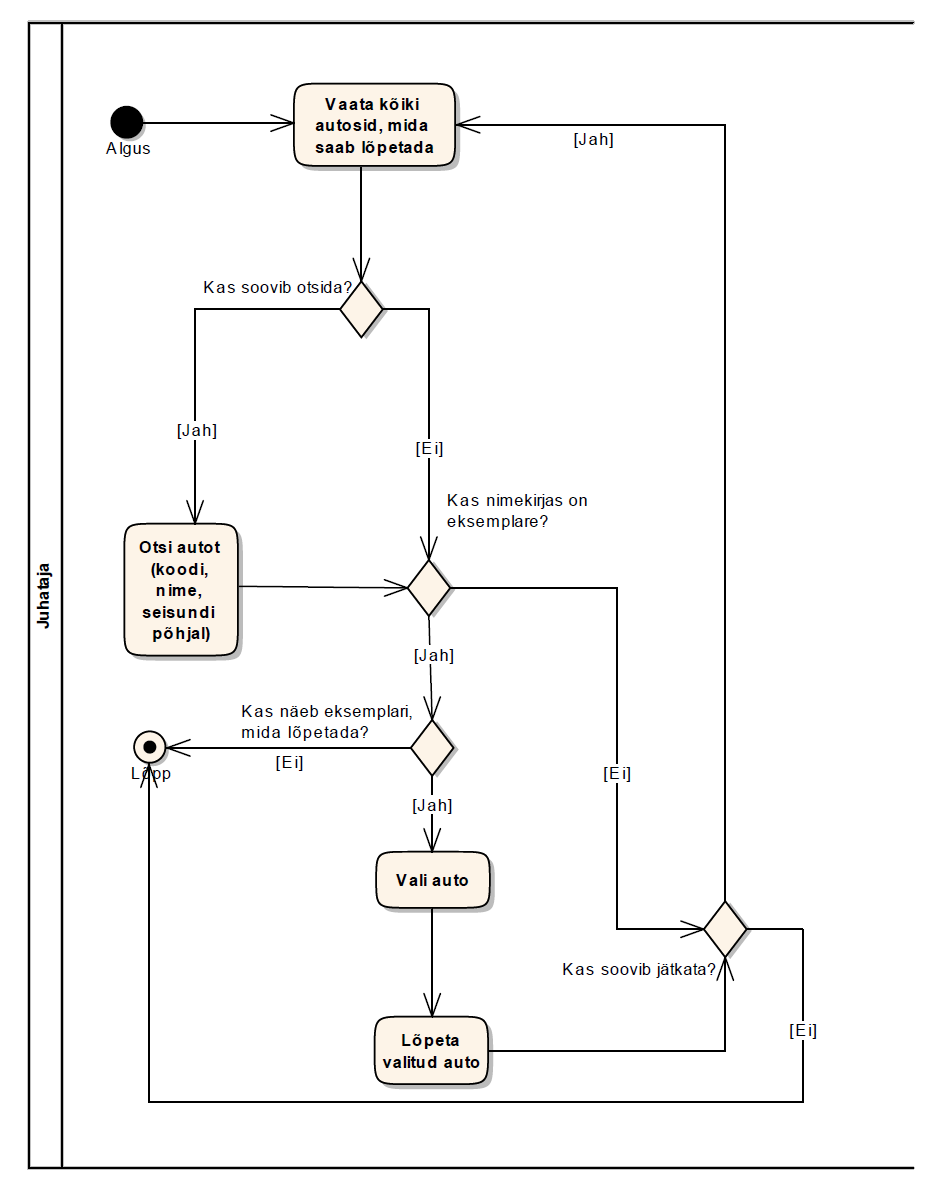
\includegraphics[scale=0.6]{joonis1}
	\caption{\textbf{Joonis 1 Auto lõpetamise tegevusdiagramm.}}
\end{figure}

\subsection{Allsüsteemi kasutusjuhtude eskiismudel}
\textbf{Joonis 2} esitatud kasutusjuhtude diagrammil on värvidel järgmine tähendus.

\begin{itemize}
	\item \colorbox{yellow}{Kollasega} on tähistatud põhikasutusjuhud.
	\item \textbf{\textcolor{orange}{Oranžiga}} on tähistatud abistavad kasutusjuhud (sisuliselt kasutusjuhu fragmendid), mis on kirja pandud selleks, et mitte kirjeldada mitmekordselt erinevates kasutusjuhtudes esinevat ühesugust funktsionaalsust.
	\item \textbf{\colorbox{light-gray}{Halliga}} on tähistatudkasutusjuhud, mis esitavad läbivaid huvisid ning on seotud rohkem kui ühe funktsionaalse allsüsteemiga.
\end{itemize}

\begin{figure}[H]
	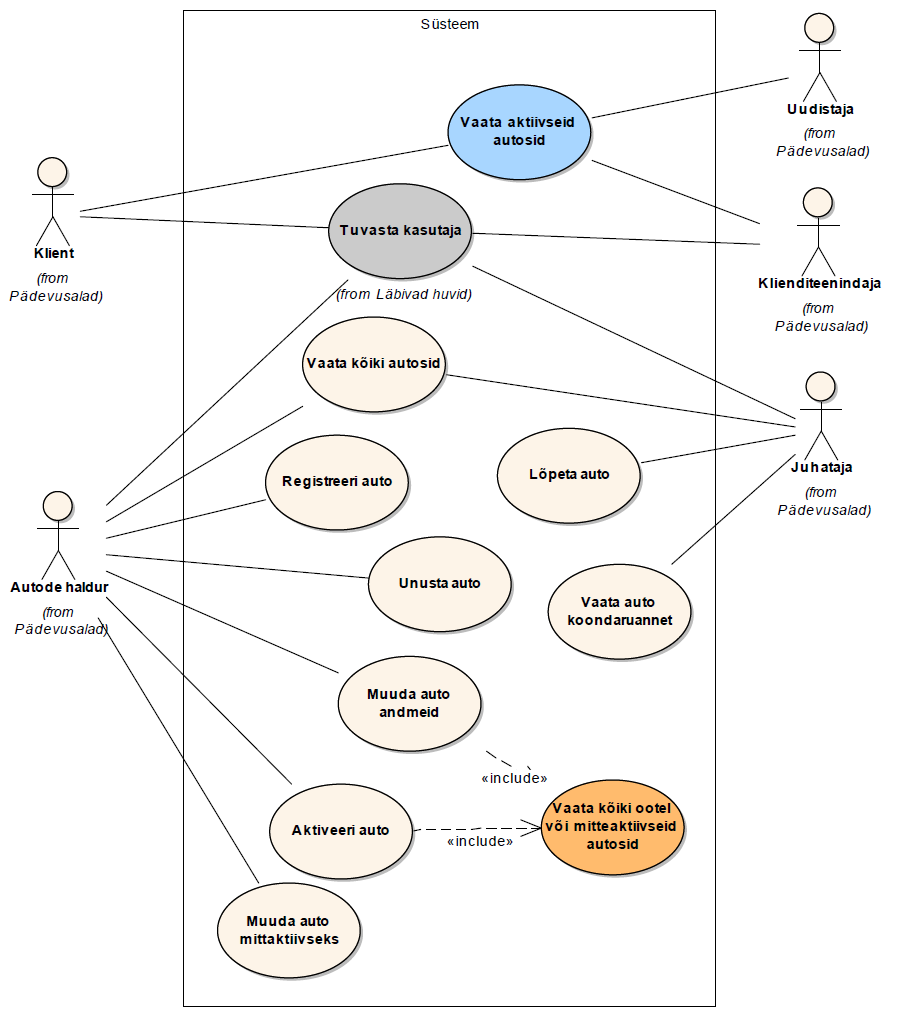
\includegraphics[scale=0.6]{joonis2}
	\caption{\textbf{Joonis 2 Auto funktsionaalse allsüsteemi kasutusjuhtude diagramm.}}
\end{figure}

\begin{flushleft}
\underline{\textbf{Kasutusjuht}: Tuvasta kasutaja} \\
\textbf{Tegutsejad}: Autode haldur, Klienditeenindaja, Juhataja, Klient – (edaspidi Subjekt) \\
\textbf{Kirjeldus}: Subjekt identifitseerib ennast. Selleks sisestab ta kasutajanime, parooli ja oma rolli süsteemis. Süsteem autendib subjekti, st kontrollib subjekti väidetavat identiteeti. Süsteemi sisenemiseks peab subjekt olema ka sobivas seisundis. Kui subjekt on autenditud (isik on tuvastatud ja identiteet kontrollitud), siis lubatakse subjekt süsteemi siseneda, vastasel juhul mitte. Lisaks autoriseeritakse subjekt, andes talle juurdepääsu infosüsteemi objektidele.
\end{flushleft}

\begin{flushleft}
\underline{\textbf{Kasutusjuht}: Registreeri auto} \\
\textbf{Tegutsejad}: Autode haldur \\
\textbf{Kirjeldus}: Autode haldur registreerib uue auto. 
\end{flushleft}

\begin{flushleft}
	\underline{\textbf{Kasutusjuht}: Unusta auto} \\
	\textbf{Tegutsejad}: Autode haldur \\
	\textbf{Kirjeldus}: Autode haldur vaatab ootel autode nimekirja, valib sealt auto ja kustutab selle andmebaasist. Subjekt saab nimekirja sorteerida ja filtreerida. 
\end{flushleft}

\begin{flushleft}
	\underline{\textbf{Kasutusjuht}: Muuda auto andmeid} \\
	\textbf{Tegutsejad}: Autode haldur \\
	\textbf{Kirjeldus}: Autode haldur vaatab ootel  või mitteaktiivsete autode nimekirja, valib sealt auto ja muudab selle andmeid. Ei ole võimalik muuta auto registreerimise aega ja infot selle kohta, kes auto registreeris. Samuti ei kuulu muudatuste hulka auto seisundi muutmine (selleks on eraldi kasutusjuhud). Samas saab muuta auto kategooriatesse kuuluvust. 
\end{flushleft}

\begin{flushleft}
	\underline{\textbf{Kasutusjuht}: Aktiveeri auto} \\
	\textbf{Tegutsejad}: Autode haldur \\
	\textbf{Kirjeldus}: Autode haldur vaatab ootel või mitteaktiivsete autode nimekirja, valib sealt auto ja muudab selle aktiivseks.  
\end{flushleft}

\begin{flushleft}
	\underline{\textbf{Kasutusjuht}: Muuda auto mitteaktiivseks} \\
	\textbf{Tegutsejad}: Autode haldur \\
	\textbf{Kirjeldus}: Autode haldur vaatab aktiivsete autode nimekirja, valib sealt auto ja muudab selle mitteaktiivseks. Subjekt saab nimekirja sorteerida ja filtreerida. 
\end{flushleft}

\begin{flushleft}
	\underline{\textbf{Kasutusjuht}: Vaata kõiki ootel või mitteaktiivseid autosid} \\
	\textbf{Tegutsejad}: Autode haldur \\
	\textbf{Kirjeldus}: Autode haldur saab vaadata nimekirja ootel või mitteaktiivses seisundis olevatest autodest. Subjekt saab nimekirja sorteerida ja filt 
\end{flushleft}

\begin{flushleft}
	\underline{\textbf{Kasutusjuht}: Vaata kõiki autosid} \\
	\textbf{Tegutsejad}: Autode haldur, Juhataja – (edaspidi Subjekt) \\
	\textbf{Kirjeldus}: Subjekt saab vaadata autode nimekirja. Subjekt saab nimekirja sorteerida ja filtreerida. Samuti saab ta iga auto korral vaadata selle detailseid andmeid. 
\end{flushleft}

\begin{flushleft}
	\underline{\textbf{Kasutusjuht}: Lõpeta auto} \\
	\textbf{Tegutsejad}: Juhataja \\
	\textbf{Kirjeldus}: Juhataja vaatab aktiivsete või mitteaktiivsete autode nimekirja, valib sealt auto ja lõpetab selle. Subjekt saab nimekirja sorteerida ja filtreerida. 
\end{flushleft}

\begin{flushleft}
	\underline{\textbf{Kasutusjuht}: Vaata autode koondaruannet} \\
	\textbf{Tegutsejad}: Juhataja \\
	\textbf{Kirjeldus}: Juhata näeb iga auto seisundi kohta selle koodi, nimetust ja selles seisundis olevate autode arvu. Kui seisundiga pole seotud ühtegi autot, siis on see arv 0. 
\end{flushleft}

\begin{flushleft}
	\underline{\textbf{Kasutusjuht}: Vaata aktiivseid autosid} \\
	\textbf{Tegutsejad}: Uudistaja, Klient, Klienditeenindaja – (edaspidi Subjekt) \\
	\textbf{Kirjeldus}: Subjekt valib kategooria ja näeb kõigi sellesse kuuluvate aktiivses seisundis olevate autode kõiki andmeid, v.a registreerimise aeg ja registreerinud töötaja. 
\end{flushleft}

\subsection{Mittefunktsionaalsed nõuded}
\begin{itemize}
	\item 
\end{itemize}

% Reduce default margins

\colorlet{shadecolor}{lightgray!20}
\newcommand{\useDash}{\renewcommand{\labelitemi}{\textendash}}

\chapter{Detailanalüüs}
Selles peatükis kirjeldatakse detailselt ja mittetehniliselt funktsionaalse allsüsteemi/registri paari, mille eskiismudelid esitati strateegilise analüüsi dokumendis.

\section{Autode funktsionaalse allsüsteemi detailanalüüs}
Järgnevalt kirjeldatakse detailselt ja mittetehniliselt autode funktsionaalse allsüsteemi toimimist.

\subsection{Kasutusjuhtude mudel}
Autode funktsionaalse allsüsteemi kasutusjuhtude diagramm (vt joonis 2).  \vspace{\pVert} \\ \hfill
\textcolor{red}{Punasega} viidatakse andmebaasioperatsioonidele, mis seisnevad ainult andmete lugemises. \textcolor{blue}{Sinisega} viidatakse andmebaasioperatsioonidele, mis tegelevad andmebaasis andmete muutmisega.

\begin{shaded}
	\subsubsection{\underline{Kasutusjuht: Tuvasta kasutaja}}
	\textbf{Primaarne tegutseja}: Autode haldur, Juhataja, Klienditeenindaja, Klient – (edaspidi Subjekt). \\
	\textbf{Osapooled ja nende huvid}:
	\useDash
	\begin{myitemize}
		\item \underline{Autode haldur, Juhataja, Klienditeenindaja, Klient}: Soovivad siseneda süsteemi ja teha tegevusi neile antud volituste piires.
	\end{myitemize}
	\textbf{Käivitav sündmus}: Subjekt soovib süsteemi siseneda. \\
	\textbf{Eeltingimused}: Subjekt on süsteemis kasutajaks registreeritud ning ta on sobivas rollis ja seisundis. \\
	\textbf{Järeltingimused}: On tehtud kindlaks, kas subjektil on õigus süsteemi siseneda või mitte. Subjekt on autenditud ja talle on antud võimalus kasutada süsteemi talle antud volituste piires (subjekt on autoriseeritud). \\
	\textbf{Stsenaarium (tüüpiline sündmuste järjestus)}:
	\begin{myenumerate}
		\item \underline{Subjekt} soovib siseneda süsteemi.
		\item \textbf{Süsteem} palub subjektil ennast identifitseerida.
		\item \underline{Subjekt} identifitseerib ennast (sisestades kasutajanime, parooli).
		\item \textbf{Süsteem} kontrollib, kas esitatud volitustõendiga (antud juhul parooliga) subjekti andmed on süsteemis olemas või mitte ning milline on tema roll ja seisund süsteemis (\textbf{\textcolor{red}{OP1.1}}).
		\item \textbf{Süsteem} annab subjektile volituse süsteemi kasutada ja annab talle juurdepääsu infosüsteemi objektidele.
	\end{myenumerate}
	\textit{Subjekt võib üritada süsteemi siseneda kuni kolm korda.} \\
	\textbf{Laiendused  (või alternatiivne sündmuste käik)}: \\
	%Formaat teine kui Erkil
	Kui süsteem ei leia esitatud volitustõendiga subjekti või pole subjekt sobivas rollis ja seisundis, siis ei saa subjekt õigust süsteemi kasutada. \\
	\indent 5a. \textbf{Süsteem} kuvab subjektile teate, et sisselogimine ebaõnnestus. Selleks, et süsteemi toimimist võimalikule ründajale mitte reeta, ei ütle süsteem täpset põhjust.
\end{shaded}

\begin{shaded}
	\subsubsection{\underline{Kasutusjuht: Registreeri auto}}
	\textbf{Primaarne tegutseja}: Autode haldur \\
	\textbf{Osapooled ja nende huvid}: 
		\useDash
		\begin{myitemize}
		\item \underline{Autode haldur}: Soovivad siseneda süsteemi ja teha tegevusi neile antud volituste piires.
		\item \underline{Juhataja}: Soovib, et organisatsiooni kasum ja klientide rahulolu oleks võimalikult suur ja selleks peab juhatajal olema ülevaade kõigist autodest ning uue auto tekkimisel ei tohi selle registreerimisega viivitada.
		\item \underline{Klient, Uudistaja}: Soovivad võimalikult täpset infot auto kohta, mida organisatsioon pakub, et otsustada, kas siduda ennast selle organisatsiooniga autot kasutava kliendi rollis.
		\end{myitemize}
	\textbf{Käivitav sündmus}: Organisatsiooni jõuab teave uue auto kohta, millega kliendid saavad hakata tulevikus tehinguid tegema. \\
	\textbf{Eeltingimused}: Autode haldur on autenditud ja autoriseeritud. \\
	\textbf{Järeltingimused}: Auto on registreeritud ja auto on seisundis "Ootel". \\
	\textbf{Stsenaarium (tüüpiline sündmuste järjestus)}:
	\begin{myenumerate}
		\item \underline{Autode haldur} avaldab soovi uus auto registreerida.
		\item \textbf{Süsteem} avab vormi, kus saab uue auto registreerida. Seal on muuhulgas võimalik määrata, millistesse kategooriatesse auto kuulub, sest süsteem pakub kategooriate valiku (\textbf{\textcolor{red}{OP2.1}}).
		\item \underline{Autode haldur} sisestab auto andmed ja valib kategooriad, millesse auto kuulub. Autode haldur ei saa registreerida auto algseisundit, registreerimise aega ning viidet registreerimise läbiviinud töötajale – seda teeb süsteem automaatselt. Ta annab korralduse salvestada.
		\item \textbf{Süsteem} salvestab auto andmed (\textbf{\textcolor{blue}{OP1}}) ning ükshaaval kõikide kategooriasse kuulumiste andmed (\textbf{\textcolor{blue}{OP7}}).
	\end{myenumerate}
	\textit{Autode haldur võib samme 1-4 läbida nii mitu korda kui soovib.} \\
	\textbf{Laiendused  (või alternatiivne sündmuste käik)}: \\
	\indent 2a. Kui ühtegi auto kategooriat pole registreeritud, siis kategooriate valikut ei pakuta ning auto kategooriasse kuulumist ei saa registreerida. \\
	\indent 3a. \underline{Autode haldur} soovib auto mõnest määratud kategooriast kohe eemaldada. \\
	\indent 3b. \textbf{Süsteem} kuvab nimekirja kategooriatest, kuhu auto juba kuulub. Iga kategooria juures on ka selle kategooria tüübi nimetus. (\textbf{\textcolor{red}{OP2.2}}) \\
	\indent 3c. \textbf{Süsteem} salvestab kategooriast eemaldamise (\textbf{\textcolor{blue}{OP8}}). \\
\end{shaded}

\begin{shaded}
	\subsubsection{\underline{Kasutusjuht: Unusta auto}}
	\textbf{Primaarne tegutseja}: Autode haldur \\
	\textbf{Osapooled ja nende huvid}: 
	\useDash
	\begin{myitemize}
		\item \underline{Autode haldur}: Soovib, et süsteemis oleks kõikide organisatsioonile teadaolevate autode andmed ja et need andmed oleksid võimalikult täpsed. Kui on selge, et autot sellisel kujul ei teki, siis soovib selle andmed segaduste vältimiseks süsteemist eemaldada.
		\item \underline{Juhataja}: Soovib, et organisatsiooni kasum ja klientide rahulolu oleks võimalikult suur ja selleks peab juhatajal olema ülevaade kõigist autodest ning uue auto tekkimisel ei tohi selle registreerimisega viivitada. Samas ei soovi ta näha autosid, millest asja ei saa.
		\item \underline{Klient, Uudistaja}: Soovivad võimalikult täpset infot autode kohta, mida organisatsioon pakub, et otsustada, kas siduda ennast selle organisatsiooniga autot kasutava kliendi rollis.
	\end{myitemize}
	\textbf{Käivitav sündmus}: Organisatsiooni jõuab teave, et autot sellisel kujul ei realiseeru ning seda ei saa hakata klientidele tehinguteks pakkuma. \\
	\textbf{Eeltingimused}: Autode haldur on autenditud ja autoriseeritud. Auto on registreeritud ja on seisundis "Ootel". \\
	\textbf{Järeltingimused}: Auto andmed on süsteemist kustutatud. \\
	\textbf{Stsenaarium (tüüpiline sündmuste järjestus)}:
	\begin{myenumerate}
		\item \underline{Autode haldur} avaldab soovi auto unustada, st selle andmed süsteemist kustutada.
		\item \textbf{Süsteem} kuvab ootel autode nimekirja, kus on auto\_kood, nimetus,  mark, mudel, valjalaske\_aasta, reg\_number, vin\_kood (\textbf{\textcolor{red}{OP3.1}}).
		\item \underline{Autode haldur} valib nimekirjast auto ja annab korralduse see unustada.
		\item \textbf{Süsteem} salvestab andmed (\textbf{\textcolor{blue}{OP2}}).
	\end{myenumerate}
	\textit{Autode haldur võib samme 1-4 läbida nii mitu korda kui soovib.} \\
	\textbf{Laiendused  (või alternatiivne sündmuste käik)}: \\
	\indent 3a. \underline{Autode haldur} saab nimekirja kõigi kuvatud väljade järgi sorteerida ja filtreerida. \\
	\indent 3b. \underline{Autode haldur} ei saa jätkata, kui nimekirjas ei ole ühtegi ootel autot.
\end{shaded}

\begin{shaded}
	\subsubsection{\underline{Kasutusjuht: Muuda auto andmeid}}
	\textbf{Primaarne tegutseja}: Autode haldur \\
	\textbf{Osapooled ja nende huvid}: 
	\useDash
	\begin{myitemize}
		\item \underline{Autode haldur}: Soovib, et süsteemis oleks kõikide organisatsioonile teadaolevate autode andmed ja et need andmed oleksid võimalikult täpsed.
		\item \underline{Juhataja}: Soovib, et organisatsiooni kasum ja klientide rahulolu oleks võimalikult suur ja selleks peab juhatajal olema täpne ülevaade kõigist autodest. 
		\item \underline{Klient, Uudistaja}: Soovivad võimalikult täpset infot autode kohta, mida organisatsioon pakub, et otsustada, kas siduda ennast selle organisatsiooniga autot kasutava kliendi rollis.
	\end{myitemize}
	\textbf{Käivitav sündmus}: Ilmneb, et autode andmete registreerimisel on tehtud viga või 
	auto atribuutide väärtuste ja seoste hulgas on toimunud muudatus (siia hulka ei kuulu seisundimuudatus, millega tegelemiseks on eraldi kasutusjuhud). \\
	\textbf{Eeltingimused}: Autode haldur on autenditud ja autoriseeritud. Auto on registreeritud ja on seisundis "Ootel" või "Mitteaktiivne". \\
	\textbf{Järeltingimused}: Auto andmed on muudetud, kuid auto seisund ning info auto registreerija ning registreerimise aja kohta ei ole muutunud. \\
	\textbf{Stsenaarium (tüüpiline sündmuste järjestus)}:
	\begin{myenumerate}
		\item \underline{Autode haldur} soovib muuta auto andmeid.
		\item \textit{Käivitub kasutusjuht "Vaata kõiki ootel või mitteaktiivseid autosid"}
		\item \underline{Autode haldur} valib nimekirjast auto ja annab korralduse vaadata selle detailseid andmeid.
		\item \textbf{Süsteem} kuvab muutmiseks mõeldud väljades auto põhiandmed  (auto\_kood, nimetus, mark, mudel, valjalaske\_aasta, mootori\_maht, auto\_kütuse\_liik, istekohtade\_arv, reg\_number, vin\_kood) (\textbf{\textcolor{red}{OP4.1}}) ning sellega seotud kategooriate ja kategooriate tüüpide nimetused (\textbf{\textcolor{red}{OP2.2}}). Seal on muuhulgas võimalik määrata, millistesse kategooriatesse auto kuulub, sest süsteem pakub kategooriate valiku (\textbf{\textcolor{red}{OP2.1}}).
		\item \underline{Autode haldur} muudab auto andmeid ja annab korralduse salvestada.
		\item \textbf{Süsteem} salvestab andmed (\textbf{\textcolor{blue}{OP6}})
	\end{myenumerate}
	\textit{Autode haldur võib samme 1-6 läbida nii mitu korda kui soovib.} \\
	\textbf{Laiendused  (või alternatiivne sündmuste käik)}: \\
	\indent 5a. \underline{Autode haldur} võib lisada auto uude kategooriasse ja anda korralduse salvestada. \\
	\indent 6a. \textbf{Süsteem} salvestab andmed (\textbf{\textcolor{blue}{OP7}}) \\
	\indent 5b. \underline{Autode haldur} võib eemaldada auto kategooriast ja anda korralduse salvestada. \\
	\indent 6b. \textbf{Süsteem} Süsteem salvestab andmed (\textbf{\textcolor{blue}{OP8}})).  \\
	\indent 5c. Kui ühtegi autode kategooriat pole registreeritud, siis kategooriate valikut ei pakuta ning auto kategooriasse kuulumist ei saa registreerida. \\
\end{shaded}

\begin{shaded}
	\subsubsection{\underline{Kasutusjuht: Aktiveeri auto}}
	\textbf{Primaarne tegutseja}: Autode haldur \\
	\textbf{Osapooled ja nende huvid}: 
	\useDash
	\begin{myitemize}
		\item \underline{Autode haldur, Juhataja}: Soovib, et iga auto kohta oleks teada tema koht üldises auto elutsüklis, mis ühtlasi määrab tegevused, mida selle autoga saab teha.
		\item \underline{Autode haldur}: Soovib, et autot saaks kasutada uutes tehingutes.
		\item \underline{Klient, Uudistaja}: Soovivad näha kõiki aktiivseid autosid, et otsustada, kas siduda ennast selle organisatsiooniga autot kasutava kliendi rollis.
	\end{myitemize}
	\textbf{Käivitav sündmus}: Auto ooteperiood või autoga seoses tekkinud ajutised probleemid on lahenenud ning auto põhjal saab uuesti tehinguid teha. \\
	\textbf{Eeltingimused}:Autode haldur on autenditud ja autoriseeritud. Auto on registreeritud ja on seisundis "Ootel" või "Mitteaktiivne". Auto on määratud vähemalt ühte auto kategooriasse.\\
	\textbf{Järeltingimused}: Auto on seisundis "Aktiivne". \\
	\textbf{Stsenaarium (tüüpiline sündmuste järjestus)}:
	\begin{myenumerate}
		\item \underline{Autode haldur} soovib aktiveerida auto.
		\item\textit{ Käivitub kasutusjuht "Vaata kõiki ootel või mitteaktiivseid autosid"}
		\item \underline{Autode haldur} valib nimekirjast auto ja annab korralduse see aktiivseks muuta.
		\item \textbf{Süsteem} salvestab andmed (\textbf{\textcolor{blue}{OP3}}).
	\end{myenumerate}
	\textit{Autode haldur võib samme 1-4 läbida nii mitu korda kui soovib.} \\
	\textbf{Laiendused  (või alternatiivne sündmuste käik)}: \\
	\indent 3a. Kui nimekirjas ei ole ühtegi ootel või mitteaktiivset autot, siis ei saa autode haldur jätkata. \\
	\indent 4a. Kui auto ei kuulu ühtegi autodekategooriasse, siis aktiveerimine ebaõnnestub.
\end{shaded}

\begin{shaded}
	\subsubsection{\underline{Kasutusjuht: Muuda auto mitteaktiivseks}}
	\textbf{Primaarne tegutseja}: Autode haldur \\
	\textbf{Osapooled ja nende huvid}: 
	\useDash
	\begin{myitemize}
		\item \underline{Autode haldur, Juhataja}: Soovib, et iga auto kohta oleks teada tema koht üldises auto elutsüklis, mis ühtlasi määrab tegevused, mida selle autoga saab teha.
		\item \underline{Autode haldur}: Soovib auto andmeid muuta või tegeleda sellega tekkinud ajutiste probleemidega, olles samal ajal veendunud, et keegi ei saa sellega algatada uusi tehinguid.
		\item \underline{Klient, Uudistaja}: Soovivad näha kõiki aktiivseid autosid, et otsustada, kas siduda ennast selle organisatsiooniga autot kasutava kliendi rollis (kui huvi pakkuv auto ei ole selles nimekirjas, siis see on talle samuti oluline informatsioon).
	\end{myitemize}
	\textbf{Käivitav sündmus}: Auto kasutamine tehingutes on vaja ajutiselt peatada kuna seoses selle autoga on ilmnenud ajutise iseloomuga probleemid. \\
	\textbf{Eeltingimused}:Autode haldur on autenditud ja autoriseeritud. Auto on registreeritud ja on seisundis "Aktiivne".\\
	\textbf{Järeltingimused}: Auto on seisundis "Mitteaktiivne". \\
	\textbf{Stsenaarium (tüüpiline sündmuste järjestus)}:
	\begin{myenumerate}
		\item \underline{Autode haldur} avaldab soovi auto mitteaktiivseks muuta.
		\item\textit \textbf{Süsteem} kuvab aktiivsete autode nimekirja, kus on auto\_kood, nimetus,  mark, mudel, valjalaske\_aasta, reg\_number, vin\_kood (\textbf{\textcolor{red}{OP6.1}}).
		\item \underline{Autode haldur} valib nimekirjast auto ja annab korralduse see mitteaktiivseks muuta.
		\item \textbf{Süsteem} salvestab andmed (\textbf{\textcolor{blue}{OP4}}).
	\end{myenumerate}
	\textit{Autode haldur võib samme 1-4 läbida nii mitu korda kui soovib.} \\
	\textbf{Laiendused  (või alternatiivne sündmuste käik)}: \\
	\indent 3a. Autode haldur saab nimekirja kõigi kuvatud väljade järgi sorteerida ja filtreerida. \\
	\indent 3b. Kui nimekirjas ei ole ühtegi aktiivset autot, siis ei saa autode haldur jätkata.
\end{shaded}

\begin{shaded}
	\subsubsection{\underline{Kasutusjuht: Vaata kõiki ootel või mitteaktiivseid autosid}}
	\textbf{Primaarne tegutseja}: Autode haldur \\
	\textbf{Osapooled ja nende huvid}: 
	\useDash
	\begin{myitemize}
		\item \underline{Autode haldur}: Soovib sisendit juhtimisotsuste tegemiseks.
	\end{myitemize}
	\textbf{Käivitav sündmus}: Subjekt soovib muuta auto andmeid, sh auto seisundit. \\
	\textbf{Eeltingimused}: Subjekt on autenditud ja autoriseeritud. \\
	\textbf{Järeltingimused}: On leitud seisundis "Ootel" või "Mitteaktiivne" olevate autode nimekiri. \\
	\textbf{Stsenaarium (tüüpiline sündmuste järjestus)}:
	\begin{myenumerate}
		\item \underline{Subjekt} soovib vaadata ootel või mitteaktiivsete autode nimekirja.
		\item\textit \textbf{Süsteem} kuvab ootel või mitteaktiivses seisundis autode nimekirja, kus on kood, nimetus, hetkeseisundi nimetus, mark, mudel, valjalaske\_aasta, reg\_number, vin\_kood (\textbf{\textcolor{red}{OP7.1}}).
	\end{myenumerate}
	\textbf{Laiendused  (või alternatiivne sündmuste käik)}: \\
	\indent 2a. Autode haldur saab nimekirja kõigi kuvatud väljade järgi sorteerida ja filtreerida. \\
\end{shaded}

\begin{shaded}
	\subsubsection{\underline{Kasutusjuht: Vaata kõiki Autosid}}
	\textbf{Primaarne tegutseja}: Autode haldur, Juhataja – (edaspidi Subjekt) \\
	\textbf{Osapooled ja nende huvid}: 
	\useDash
	\begin{myitemize}
		\item \underline{Autode haldur, Juhataja}: Soovib sisendit juhtimisotsuste tegemiseks.
	\end{myitemize}
	\textbf{Käivitav sündmus}: Subjekt tahab mingil põhjusel vaadata autode detailseid andmeid (sealhulgas juba lõpetatud autode andmeid). Näiteks soovib subjekt näha, milliseid autosid on organisatsioon kunagi pakkunud või milliseid see praegu pakub. \\
	\textbf{Eeltingimused}:Subjekt on autenditud ja autoriseeritud.\\
	\textbf{Järeltingimused}: On leitud kõikide autode detailsed andmed. \\
	\textbf{Stsenaarium (tüüpiline sündmuste järjestus)}:
	\begin{myenumerate}
		\item \underline{Subjekt} soovib vaadata kõikide autode andmeid.
		\item\textit \textbf{Süsteem} kuvab kõigi autode nimekirja, kus on kood, nimetus, hetkeseisundi nimetus, mark, mudel, valjalaske\_aasta, reg\_number, vin\_kood (\textbf{\textcolor{red}{OP8.1}}).
		\item \underline{Subjekt} valib auto, mida ta soovib detailsemalt vaadata.
		\item \textbf{Süsteem} kuvab vaatamiseks mõeldud väljades auto põhiandmed andmed (auto\_kood, nimetus, mark, mudel, valjalaske\_aasta, mootori\_maht, auto\_kütuse\_liik, istekohtade\_arv, reg\_number, vin\_kood, registreerimise aeg, registreerinud töötaja eesnimi, perenimi ja e-meili aadress) (\textbf{\textcolor{red}{OP8.2}}) ning sellega seotud kategooriate ja kategooriate tüüpide nimetused (\textbf{\textcolor{red}{OP2.2}}).
	\end{myenumerate}
	\textbf{Laiendused  (või alternatiivne sündmuste käik)}: \\
	\indent 3a. Subjekt saab nimekirja kõigi kuvatud väljade järgi sorteerida ja filtreerida. \\
	\indent 3b. Kui nimekirjas ei ole ühtegi autot, siis ei saa subjekt jätkata.
\end{shaded}

\begin{shaded}
	\subsubsection{\underline{Kasutusjuht: Lõpeta auto}}
	\textbf{Primaarne tegutseja}: Juhataja \\
	\textbf{Osapooled ja nende huvid}: 
	\useDash
	\begin{myitemize}
		\item \underline{Autode haldur, Juhataja}: Soovib, et iga auto kohta oleks teada tema koht üldises auto elutsüklis, mis ühtlasi määrab tegevused, mida selle autoga saab teha.
		\item \underline{Juhataja}: Soovib anda kõigile huvitatud osapooltele teada, et autoga enam tehinguid ei tehta (kuid kõik käimasolevad tehingud tuleb vastavalt kehtivale korrale lõpetada). Samas soovib ta auto andmete süsteemis säilimist, et ei läheks kaotsi info auto ja sellega seotud tehingute kohta.
		\item \underline{Klient, Uudistaja}: Soovivad näha kõiki aktiivseid autosid, et otsustada, kas siduda ennast selle organisatsiooniga autot kasutava kliendi rollis (kui huvi pakkuv auto ei ole selles nimekirjas, siis see on talle samuti oluline informatsioon).
	\end{myitemize}
	\textbf{Käivitav sündmus}: Auto kasutamine tehingutes on vaja püsivalt lõpetada, kuna seoses autoga on ilmnenud püsiva iseloomuga probleemid või kuna auto on oma aja lihtsalt ära elanud. \\
	\textbf{Eeltingimused}:Juhataja on autenditud ja autoriseeritud. Auto on registreeritud ja on seisundis "Aktiivne" või "Mitteaktiivne".\\
	\textbf{Järeltingimused}: Auto seisund on muutunud "Lõpetatud", kuid auto andmed on süsteemis endiselt alles. Auto andmeid ei tohi süsteemist füüsiliselt kustutada, sest sellega seoses tuleks kustutada info kõigi tehingute kohta, millega auto on seotud. \\
	\textbf{Stsenaarium (tüüpiline sündmuste järjestus)}:
	\begin{myenumerate}
		\item \underline{Juhataja} avaldab soovi auto lõpetada.
		\item\textit \textbf{Süsteem} kuvab aktiivsete või mitteaktiivsete autode nimekirja, kus on kood, nimetus,  hetkeseisundi nimetus, mark, mudel, valjalaske\_aasta, reg\_number, vin\_kood (\textbf{\textcolor{red}{OP9.1}}).
		\item \underline{Juhataja} valib nimekirjast auto ja annab korralduse see lõpetada.
		\item \textbf{Süsteem} salvestab andmed (\textbf{\textcolor{blue}{OP5}}).
	\end{myenumerate}
	\textit{Juhataja võib samme 1-4 läbida nii mitu korda kui soovib. }\\
	\textbf{Laiendused  (või alternatiivne sündmuste käik)}: \\
	\indent 3a. Juhataja saab nimekirja kõigi kuvatud väljade järgi sorteerida ja filtreerida. \\
	\indent 3b. Kui nimekirjas ei ole ühtegi aktiivset või mitteaktiivset autot, siis ei saa juhataja jätkata.
\end{shaded}

\begin{shaded}
	\subsubsection{\underline{Kasutusjuht: Vaata auto koondaruannet}}
	\textbf{Primaarne tegutseja}: Juhataja \\
	\textbf{Osapooled ja nende huvid}: 
	\useDash
	\begin{myitemize}
		\item \underline{Autode haldur}: Soovib sisendit juhtimisotsuste tegemiseks.
		\item \underline{Autode haldur}: Soovib, et juhataja teeks häid otsuseid ja äri kestaks.
	\end{myitemize}
	\textbf{Käivitav sündmus}: Juhataja soovib juhtimisotsuste tegemiseks seada, kui palju on iga auto elutsükli seisundi kohta autosid, mis on parajasti selles seisundis. \\
	\textbf{Eeltingimused}: Juhataja on autenditud ja autoriseeritud. Auto seisundi liigid on registreeritud. \\
	\textbf{Järeltingimused}: Auto koondaruanne on moodustatud. \\
	\textbf{Stsenaarium (tüüpiline sündmuste järjestus)}:
	\begin{myenumerate}
		\item \underline{Juhataja} soovib vaadata auto koondaruannet.
		\item\textit \textbf{Süsteem} kuvab iga auto elutsükli seisundi kohta selle seisundi koodi, nimetuse (suurtähtedega) ja hetkel selles seisundis olevate autode arvu. Kui selles seisundis pole hetkel ühtegi autot, siis on arv 0. Seisundid on sorteeritud autode arvu järgi kahanevalt. Kui mitmel seisundil on samasugune autode arv, siis need on sorteeritud suurtähtedega nime järgi tähestiku järjekorras (\textbf{\textcolor{red}{OP10}}).
	\end{myenumerate}
	\textbf{Laiendused  (või alternatiivne sündmuste käik)}: \\
	\indent 2a. Kui ükski auto seisundi liik pole registreeritud, siis ei saa olla ka registreeritud mitte ühtegi autot ja sellisel juhul tagastab päring null rida. \\
\end{shaded}

\begin{shaded}
	\subsubsection{\underline{Kasutusjuht: Vaata aktiivseid autosid}}
	\textbf{Primaarne tegutseja}: Uudistaja, Klient, Klienditeenindaja – (edaspidi Subjekt). \\
	\textbf{Osapooled ja nende huvid}: 
	\useDash
	\begin{myitemize}
		\item \underline{Autode haldur, Juhataja, Klienditeenindaja}:Tahavad, et võimalikel huvilistel oleks täpne ülevaade organisatsiooni pakutavast ja et see kallutaks neid organisatsiooni kliendiks hakkama.õ
		\item \underline{Klient, Uudistaja}: Soovivad näha organisatsiooni pakutavate autode nimekirja, et langetada tarbimisotsuseid.
	\end{myitemize}
	\textbf{Käivitav sündmus}: Subjekt tunneb huvi organisatsiooni poolt hetkel pakutavate autode kohta, et otsustada, kas ennast tulevikus organisatsiooniga tihedamalt siduda. \\
	\textbf{Eeltingimused}:Klient on autenditud ja autoriseeritud, uudistaja ei ole autenditud ja autoriseeritud.\\
	\textbf{Järeltingimused}: Aktiivsete autode nimekiri on leitud. \\
	\textbf{Stsenaarium (tüüpiline sündmuste järjestus)}:
	\begin{myenumerate}
		\item \underline{Subjekt} soovib näha kõiki organisatsiooni pakutavaid aktiivseid autosid.
		\item\textit \textbf{Süsteem} kuvab nimekirja kategooriatest (\textbf{\textcolor{red}{OP2.1}}).
		\item \underline{Subjekt} valib konkreetse kategooria.
		\item \textbf{Süsteem} kuvab sellesse kuuluvate aktiivsete autode nimekirja. Iga auto kohta esitatakse kood, nimetus, kategooriate ja nende tüüpide nimetused, valjalaske\_aasta, mark, mudel, istekohtade arv, mootori maht, kütuse liik  (\textbf{\textcolor{blue}{OP11.2}}).
	\end{myenumerate}
	\textit{Juhataja võib samme 1-4 läbida nii mitu korda kui soovib. }\\
	\textbf{Laiendused  (või alternatiivne sündmuste käik)}: \\
	\indent 4a. Kui pole ühtegi aktiivset autot, siis on nimekiri tühi. \\
	\indent 4b. Subjekt võib vaadatavate autode hulka koodi ja nimetuse järgi sorteerida ning filtreerida.
\end{shaded}

\section{Autode funktsionaalse allsüsteemi vajatavate registrite detailanalüüs}
Järgnevalt kirjeldatakse detailselt ja mittetehniliselt autode funktsionaalse allsüsteemi vajatavate registrite struktuuri ja toimimist.

\subsection{Kontseptuaalne andmemudel}
Järgnevalt esitatakse kontseptuaalne andmemudel, mis koosneb olemi suhte diagrammidest ja nendel olevate olemitüüpide ja atribuutide sõnalistest kirjeldustest.  \vspace{\pVert} \\ \hfill

Joonis  esitatud olemi suhte diagrammidel on värvidel järgmine tähendus.
\begin{itemize}
	\item \textcolor{red}{Punasega} on tähistatud autode registri põhiobjekt.
	\item \hl{Kollasega} on tähistatud autode registrisse kuuluvad mitte-põhiobjektid.
	\item \textcolor{green}{Rohelisega} on tähistatud teistesse registritesse kuuluvad objektid, mida on antud juhul vaja autode funktsionaalse allsüsteemi toimimise tagamiseks.
\end{itemize}

\begin{figure}[H]
	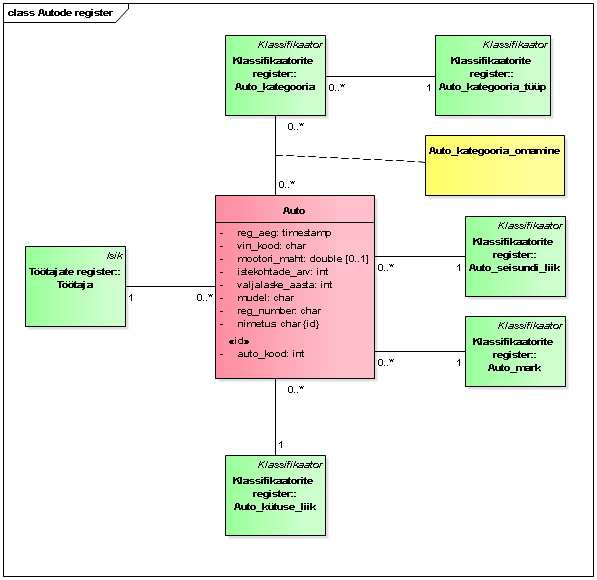
\includegraphics[scale=1]{joonis5}
	\caption{\textbf{Joonis 5 Auto registri olemi-suhte diagramm.}}
\end{figure}

\begin{figure}[H]
	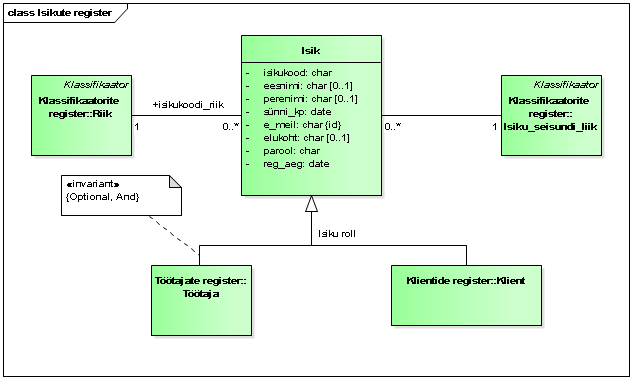
\includegraphics[scale=1]{joonis6}
	\caption{\textbf{Joonis 6 Isikute registri olemi-suhte diagramm.}}
\end{figure}

\begin{figure}[H]
	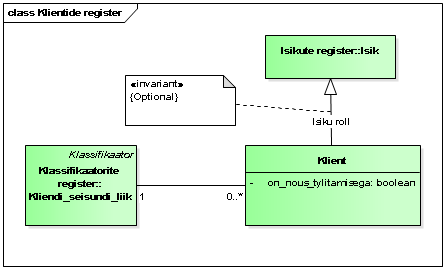
\includegraphics[scale=1]{joonis7}
	\caption{\textbf{Joonis 7 Klientide registri olemi-suhte diagramm.}}
\end{figure}

\begin{figure}[H]
	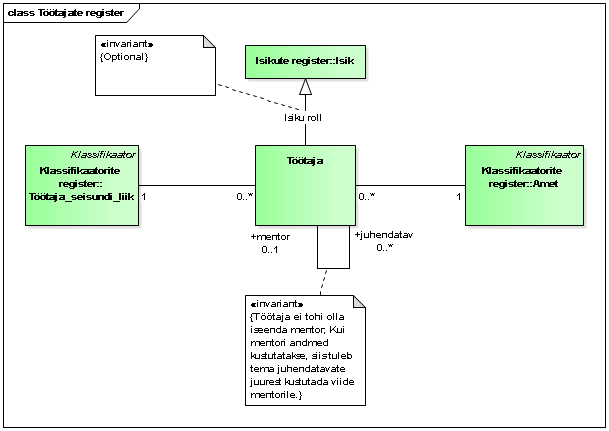
\includegraphics[scale=1]{joonis8}
	\caption{\textbf{Joonis 8 Töötajate registri olemi-suhte diagramm.}}
\end{figure}

\begin{figure}[H]
	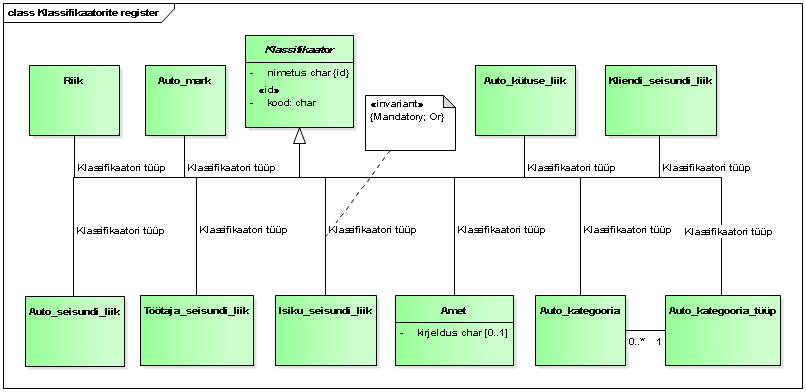
\includegraphics[scale=1]{joonis9}
	\caption{\textbf{Joonis 9 Laiendatud auto registri olemi-suhte diagrammid.}}
\end{figure}

Tabel 5 esitab olemi-suhte diagrammidel esitatud olemitüüpide sõnalised kirjeldused.

\begin{longtabu} to \textwidth {| X | X | X[2] |} 
	\caption{\textbf{Tabel 5 Olemitüüpide sõnalised kirjeldused.}} \\
	% -----------------headings----------------------%
	\hline
	\rowcolor[HTML]{C0C0C0}
	\textbf{Olemitüübi nimi (teised nimed)}   &   \textbf{Kuuluvus registrisse} & \textbf{Definitsioon} \\
	\hline
	\endfirsthead
	%headings for next page columns
	\hline
	\rowcolor[HTML]{C0C0C0}
	\textbf{Olemitüübi nimi (teised nimed)}   &   \textbf{Kuuluvus registrisse} & \textbf{Definitsioon} \\
	\hline
	\endhead
	% ---------------headings end--------------------%
	Amet
	& Klassifikaatorite register
	& Amet on töölepingus sätestatud ametikohustuste üldnimetus. Ametid on klassifikaatorid. Näited on juhataja ja klienditeenindaja. \\ \hline
	
	Auto
	& Autode register
	& Auto on sõiduvahend, mis on organisatsioonis varana arvel ning millega sooritatakse tehinguid organisatsiooni klientidega. „Auto on vähemalt kolmerattaline ja kaheteljeline mootorsõiduk reisijate või veoste vedamiseks rööpmeta teedel või maastikul.“ (Vikipeedia) Auto all mõeldakse sõiduautot. „Sõiduautodeks loetakse tavaliselt reisijate vedamiseks mõeldud väiksemaid, 2–9[viide?]-kohalisi autosid.“ (Vikipeedia) \\ \hline
	
	Auto\_kategooria
	& Klassifikaatorite register
	& Võimaldab auto klassifitseerimist erinevatesse kategooriatesse ja selle alusel autode rühmitamist teatud põhjusel huvipakkuvateks hulkadeks. Tegemist on üksteist mittevälistavate kategooriatega, st üks ja sama auto võib kuuluda korraga mitmesse sama tüüpi kategooriasse. Näited on pereauto ja väikeauto. \\ \hline
	
	Auto\_kategooria\_omamine
	& Autode register
	& Näitab auto kuulumist kategooriatesse. Iga auto ja iga auto kategooria vahel võib olla maksimaalselt üks seos. \\ \hline
	
	Auto\_kategooria\_tüüp
	& Klassifikaatorite register 
	& Võimaldab rühmitada auto klassifitseerimiseks kasutatavaid kategooriaid ühise nime alla. Need nimed kirjeldavad, mis liiki klassifikatsiooniga on tegemist. Näide on sihtgrupp. \\ \hline
	
	Auto\_kütuse\_liik
	& Klassifikaatorite register 
	& Võimaldab auto klassifitseerimist kütuseliigi alusel. Näited on bensiin ja diisel. \\ \hline
	
	Isik
	& Isikute register 
	& Mistahes organisatsiooniga seotud füüsiline isik (eraisik). Isik võib olla seotud organisatsiooniga näiteks kui klient või kui töötaja. \\  \hline
		
	Isiku\_seisundi\_liik
	& Klassifikaatorite register 
	& Seisundiklassifikaator, mis võimaldab fikseerida iga isiku puhul tema hetkeseisundi vastavalt üldisele isikute elutsüklile. Näited on elus ja surnud. \\ \hline
	
	Klassifikaator
	& Klassifikaatorite register 
	& Klassifikaatorid on "mistahes andmed, mida kasutatakse andmebaasis teiste andmete liigitamiseks või andmebaasis olevate andmete seostamiseks väljaspool organisatsiooni vastutusala oleva informatsiooniga." (Chisholm, 2000) \\ \hline

	Kliendi\_seisundi\_liik
	& Klassifikaatorite register 
	& Seisundiklassifikaator, mis võimaldab fikseerida iga kliendi puhul tema hetkeseisundi vastavalt üldisele kliendi elutsüklile. Näited on aktiivne ja mustas nimekirjas. \\ \hline
	
	Klient
	& Klientide register 
	& Organisatsioonis end kliendina registreerinud isik, kellel on võimalik osta organisatsiooni poolt pakutavaid tooteid või teenuseid. \\ \hline
	
	Riik
	& Klassifikaatorite register 
	& "Riik on kindla territooriumiga sõltumatu (suveräänne) üksus (juriidiline lähenemine).“ (Vikipeedia) Riikidena käsitletakse riike ja territooriumeid, mis on kirjeldatud Eesti Statistika lehel olevas riikide ja territooriumite klassifikaatori dokumendis, mis on omakorda eestindatud versioon rahvusvahelisest standardist "International Standard Codes for the Representation of the Names of Countries (ISO 3166) \\ \hline
	
	Töötaja
	& Töötajate register
	& Organisatsioonis (kui tööandja juures) töölepingu alusel töötav ja selle organisatsiooni juhtimisele ning kontrollile alluv isik, kes saab oma töö eest töölepingus kokkulepitud tasu. \\ \hline
	
	Töötaja\_seisundi\_liik
	& Klassifikaatorite register
	& Seisundiklassifikaator, mis võimaldab fikseerida iga töötaja puhul tema hetkeseisundi vastavalt üldisele töötajate elutsüklile. Näited on tööl ja puhkusel. \\ \hline
	\end{longtabu}

Tabel 6 esitab atribuutide sõnalised kirjeldused.

\begin{longtabu} to \textwidth {| X | X | X[2] | X |} 
	\caption{\textbf{Tabel 6 Atribuutide sõnalised kirjeldused.}} \\
	% -----------------headings----------------------%
	\hline
	\rowcolor[HTML]{C0C0C0}
	\textbf{Olemitüübi nimi}   &   \textbf{Atribuudi nimi (teised nimed)} & \textbf{Atribuudi definitsioon}  & \textbf{Näiteväärtus} \\
	\hline
	\endfirsthead
	%headings for next page columns
	\hline
	\rowcolor[HTML]{C0C0C0}
	\textbf{Olemitüübi nimi}   &   \textbf{Atribuudi nimi (teised nimed)} & \textbf{Atribuudi definitsioon}  & \textbf{Näiteväärtus} \\
	\hline
	\endhead
	% ---------------headings end--------------------%

	Amet
	& kirjeldus
	& Ametist tulenevate õiguste ja kohustuste vabatekstiline kirjeldus.
	
	\textbf{Kirjeldus ei tohi olla tühi string või ainult tühikutest koosnev string. Kasutage andmetüüpi, mis võimaldab suurimat võimalikku stringi pikkust.}
	& Juhib organisatsiooni igapäevast tööd ning langetab strateegilisi otsuseid 
	 \\ \hline
	
	Auto
	& auto\_kood
	& Auto arvuline kood, mis sisestatakse inimkasutaja poolt, mitte ei genereerita süsteemi poolt. 
	
	\textbf{Auto unikaalne identifikaator. Registreerimine on kohustuslik}
	& 222
	\\ \hline
	
   	Auto
	& nimetus (hüüdnimi)
	& Auto hüüdnimi, millega sellele äratuntavalt viidata.
	
	\textbf{Auto unikaalne identifikaator. Võib olla kuni 50 märki. Registreerimine on kohustuslik. Nimetus ei tohi olla tühi string ega ainult tühikutest koosnev string.}
	& Nimetus\\ \hline
	
   	Auto
	& reg\_aeg
	& Auto registreerimise aeg kuupäeva ja kellaaja täpsusega. Selle võib süsteem ise automaatselt määrata.
	
	\textbf{Registreerimine on kohustuslik. Väärtus peab olema vahemikus 01. jaanuar 2010 00:00:00 ja 31. detsember 2100 kell 23:59:59 (otspunktid kaasa arvatud).}
	
	& 22.03.2015 12:33\\ \hline
	
   	Auto
	& valjalaske\_
	aasta
	& Auto tootmisaasta.
	
	\textbf{Registreerimine on kohustuslik.
	Väärtus peab olema vahemikus 2000 – 2100 (otspunktid kaasa arvatud).}
	& 2009\\ \hline
	
   	Auto
	& istekohtade\_arv
	& Auto istekohtade arv.
	
	\textbf{Registreerimine on kohustuslik.}
	\textbf{Väärtus peab olema vahemikus 2 kuni 11 (otspunktid kaasa arvatud).}
	& 4\\ \hline
	
   	Auto
	& mudel
	& Auto mudel. Mudel on autotootja poolt kasutatav nimi, et kirjeldada ja reklaamida ühesuguste omadustega autosid.
	
	\textbf{Registreerimine on kohustuslik. Mudel ei tohi olla tühi string ega tühikutest koosnev string.}
	& A4\\ \hline
	
   	Auto
	& mootori\_maht
	& Auto mootori maht liitrites. 
	
	\textbf{Registreerimine on kohustuslik. Ei tohi olla negatiivne arv. Kümnendmurd täpsusega üks koht peale koma.}
	& 2.5\\ \hline
	
   	Auto
	& reg\_number (registreerimismärk, registrinumber)
	& Eesti autoregistri poolt väljastatud registreerimisnumber. Erinevatel autodel võib erinevatel aegadel olla sama number.
	
	\textbf{Registreerimine on kohustuslik.}
		
	\textbf{Ei tohi leiduda kahte aktiivses seisundis  autot, millel on sama registrinumber, st aktiivsete autode registrinumbrid peavad olema unikaalsed.}
	
	\textbf{Registrinumber ei tohi olla tühi string ega tühikutest koosnev string. Registrinumbris on lubatud suurtähed ja numbrid. Märkide hulk peab olema 2-9 (otspunktid kaasa arvatud). Registrinumber peab järgima ühte järgmistest mustritest.}
	
	\textbf{1.	Üks või rohkem suurtähte, millele järgneb üks või rohkem numbrit.
	2.	Kaks või kolm numbrit, millele järgneb kolm suurtähte.}
	& QWE321\\ \hline
	
   	Auto
	& vin\_kood
	& Tehase poolt väljastatud unikaalne auto kood.
	
	\textbf{Auto unikaalne identifikaator. Registreerimine on kohustuslik. Vin kood peab olema 11-17 märki (otspunktid kaasa arvatud) ning tohib sisaldada ainult numbreid ja suurtähti.}
	& WAUFFAFM3CA000000\\ \hline
	
   	Isik
	& isikukood
	& Riigi poolt väljastatud isiku identifikaator, mis on unikaalne selle väljastanud riigi piires.
	
	\textbf{Registreerimine on kohustuslik. Koos riigi identifikaatoriga on isiku unikaalne identifikaator.Isikukoodis on lubatud tähed, numbrid, tühikud, sidekriipsud ja / 
	Isikukood ei tohi olla tühi string või ainult tühikutest koosnev string.}
	& 39204010231\\ \hline
	
   	Isik
	& eesnimi
	& "Lapsele pärast sündi (registreerimisel) pandav nimi, osa isikunimest. Eesnimi asetseb harilikult perekonnanime ees, harva järel (nt Ungari pruugis)." (ESTERM)
	
	\textbf{Vähemalt üks kahest – eesnimi või perenimi peab olema registreeritud. Eesnimi ei tohi olla tühi string või ainult tühikutest koosnev string.}
	& Mart\\ \hline
	
   	Isik
	& perenimi (perekonna- nimi)
	& "Nimi, mis on isikul ühine teiste tema perekonna liikmetega" (ESTERM)
	
	\textbf{Vähemalt üks kahest – eesnimi või perenimi peab olema registreeritud. Perenimi ei tohi olla tühi string või ainult tühikutest koosnev string.}
	& Mets\\ \hline
	
   	Isik
	& sünni\_kp
	& Isiku sünni kuupäev sünnikoha kohaliku aja järgi.
	
	\textbf{Registreerimine on kohustuslik. Sünni kuupäeva võimalikud väärtused on vahemikus 01. jaanuar 1900 ja 31. detsember 2100 (otspunktid kaasa arvatud). Sünni kuupäev ei tohi olla suurem isiku registreerimise ajast.}
	& 12.08.1993\\ \hline
	
   	Isik
	& elukoht
	& Isiku alalise elukoha aadress. 
	
	"Koha-aadress on territooriumi haldusjaotuse hierarhiast ja ametlikest kohanimedest lähtuv aadressobjekti tekstilis-numbriline kirje või tunnus. Ühele objektile võib määrata mitu koha-aadressi. Ühele objektile määratud koha-aadressid on paralleelaadressid." ("Aadressandmete süsteemi kehtestamine")	
	
	\textbf{Elukoht ei tohi olla tühi string, ainult tühikutest koosnev string või ainult numbritest koosnev string.}
	& Tallinn, 34124, Ehitajate tee 62-12. Harjumaa, Viimsi vald, Kaku küla, Laane talu.\\ \hline
	
   	Isik
	& e\_meil (e\_mail, meil, meiliaadress, e-posti aadress)
	& Aadress, millele saab  üle võrgu (ühest arvutist või tööjaamast teise) saata isikule mõeldud kirjalikke sõnumeid. Kasutatakse kasutaja tuvastamisel kasutajanimena. 
	
	\textbf{Registreerimine on kohustuslik. Isiku tõstutundetud unikaalne identifikaator. Teiste sõnadega, kui süsteemis on näiteks meiliaadress Mati@mets.ee, siis meiliaadressi mati@mets.ee lisada ei saa.}
		
	\textbf{e\_meil peab sisaldama täpselt ühte "@" märki. Võib olla kuni 254 märki pikk.}
	& kalamees@hot.ee\\ \hline
	
   	Isik
	& parool
	& Isiku identsust tõendav teadmuslik (miski, mida isik teab) volitustõend. Andmebaasis salvestatakse parooli ja soola põhjal leitud räsiväärtus.
	
	\textbf{Registreerimine on kohustuslik.}
	& \$2a\$11\$FsKdoFDJePwuYtyg2hBxz.e8AwSODaO/nFGGacEm05vIgOBNG9dHC\\ \hline
	
	Isik
	& reg\_aeg
	& Isiku registreerimise aeg kuupäeva ja kellaaja täpsusega. Selle võib süsteem ise automaatselt määrata.
	
	\textbf{Registreerimine on kohustuslik. Väärtus peab olema vahemikus 01. jaanuar 2010 00:00:00 ja 31. detsember 2100 kell 23:59:59 (otspunktid kaasa arvatud).}
	& 12.08.2014 17:01\\ \hline
	
	Klassifikaator
	& kood
	& Klassifikaatori väärtust esitav kood, mida saab kasutada selle väärtuse lühidalt esitamiseks. Kood võib olla tekstiline või numbriline väärtus. Kood peaks olema võimalikult hästi meeldejääv. See tähendab, et kui kasutaja näeb koodi, siis seostub see tema jaoks võimalikult lihtsalt koodiga iseloomustatava klassifikaatori väärtusega.
	
	\textbf{Klassifikaatori unikaalne identifikaator, mis on unikaalne klassifikaatori tüübi piires. Registreerimine on kohustuslik.}
		
	\textbf{Riikide koodid koosnevad vastavalt ISO 3166 standardile täpselt kolmest suurtähest.}
	
	\textbf{Kui kood on tekstiline väärtus, siis ei tohi see olla tühi string või ainult tühikutest koosnev string.}
	& EST\\ \hline
	
	Klassifikaator
	& nimetus
	& Klassifikaatori väärtuse ametlik nimetus. Riikide nimetused leitakse Eesti Statistika kodulehelt alajaotusest Riikide ja territooriumide klassifikaator 2013v1.
	
	\textbf{Klassifikaatori unikaalne identifikaator, mis on unikaalne klassifikaatori tüübi piires.  Erandiks on Auto\_kategooria nimetus, mis peab olema unikaalne kombinatsioonis Auto\_kategooria\_tüübiga, st erinevat tüüpi kategooriates võib olla sama nimetusega kategooriaid.}
		
	\textbf{Registreerimine on kohustuslik. Nimetus ei tohi olla tühi string või
	ainult tühikutest koosnev string.}
	
	& Aktiivne\\ \hline
	
	Klassifikaator
	& on\_nous\_tylitamisega
	& Kirjeldab ära kas klient on nõus saama organisatsiooni poolt saadetavaid reklaamkirju 
	
	\textbf{Registreerimine on kohustuslik. Vaikeväärtus on 'False'.}
	& True\\ \hline
	\end{longtabu}

\subsection{Andmebaasioperatsioonide lepingud}
\textbf{\textcolor{blue}{OP1} Registreeri auto (p\_auto\_kood, p\_nimetus, p\_valjalaske\_aasta, p\_istekohtade\_arv, p\_mudel, p\_mootori\_maht, p\_reg\_number, töötaja identifikaator, kütuse liik identifikaator, mark identifikaator)} \\
\textbf{Eeltingimused:}
\begin{itemize}
	\item Auto\_seisundi\_liik eksemplar asl (millel on nimetus="Ootel") on registreeritud
	\item Auto\_kütuse\_liik eksemplar akl (millel on kütuse liik identifikaator) on registreeritud
	\item Auto\_mark eksemplar am (millel on mark identifikaator) on registreeritud
	\item Töötaja eksemplar t (millel on töötaja identifikaator) on registreeritud
\end{itemize}
\textbf{Järeltingimused:} \\
\textcolor{green}{--Loo eksemplare}
\begin{itemize}
	\item Auto eksemplar a on registreeritud
\end{itemize}
\textcolor{green}{--Väärtusta atribuute}
\begin{itemize}
	\item a.auto\_kood:= p\_auto\_kood
	\item a.nimetus:= p\_nimetus
	\item a.reg\_aeg:= hetke kuupäev + kellaaeg
	\item a. valjalaske\_aasta:= p\_ valjalaske\_aasta
	\item a.istekohtade\_arv:= p\_istekohtade\_arv
	\item a.mudel:= p\_mudel
	\item a.mootori\_maht:= p\_mootori\_maht
	\item a.reg\_number:= p\_reg\_number
	\item a.vin\_kood:= p\_vin\_kood
\end{itemize}
\textcolor{green}{--Loo seoseid}
\begin{itemize}
	\item a ja asl seos on registreeritud
	\item a ja t seos on registreeritud
	\item a ja akl seos on registreeritud
	\item a ja am seos on registreeritud
\end{itemize}
\textbf{Kasutus kasutusjuhtude poolt:} Registreeri auto \\ \hfill

\textbf{\textcolor{blue}{OP2} Unusta auto(p\_auto\_kood)}
\textbf{Eeltingimused:}
\begin{itemize}
	\item Auto eksemplar a (millel on auto\_kood=p\_auto\_kood) on registreeritud
	\item a on seotud auto\_seisundi\_liik eksemplariga asl (millel on nimetus="Ootel")
\end{itemize}
\textbf{Järeltingimused:} \\
\textcolor{green}{--Kustuta eksemplare ja seoseid}
\begin{itemize}
	\item a ja kõik selle seosed on andmebaasist kustutatud 
\end{itemize}
\textbf{Kasutus kasutusjuhtude poolt:} Unusta auto \\ \hfill

\textbf{\textcolor{blue}{OP3} Aktiveeri Auto (p\_auto\_kood)}
\textbf{Eeltingimused:}
\begin{itemize}
	\item Auto eksemplar a (millel on auto\_kood=p\_auto\_kood) on registreeritud
	\item a on seotud auto\_seisundi\_liik eksemplariga asl\_vana (millel on nimetus="Ootel") või (nimetus="Mitteaktiivne")
	\item auto\_seisundi\_liik eksemplar asl\_uus (millel on nimetus="Aktiivne") on registreeritud
	\item Leidub vähemalt üks auto\_kategooria\_omamine eksemplar ako, mis on seotud a-ga
\end{itemize}
\textbf{Järeltingimused:} \\
\textcolor{green}{--Kustuta seoseid}
\begin{itemize}
	\item a ja asl\_vana seos on kustutatud
\end{itemize}
\textcolor{green}{--Loo seoseid}
\begin{itemize}
	\item a ja asl\_uus seos on registreeritud
\end{itemize}
\textbf{Kasutus kasutusjuhtude poolt:} Aktiveeri auto \\ \hfill

\textbf{\textcolor{blue}{OP4} Muuda auto mitteaktiivseks autoks(p\_auto\_kood)}
\textbf{Eeltingimused:}
\begin{itemize}
	\item Auto eksemplar a (millel on auto\_kood=p\_auto\_kood) on registreeritud
	\item a on seotud auto\_seisundi\_liik eksemplariga asl\_vana (millel on nimetus="Aktiivne")
	\item auto\_seisundi\_liik eksemplar asl\_uus (millel on nimetus="Mitteaktiivne") on 
\end{itemize}
\textbf{Järeltingimused:} \\
\textcolor{green}{--Kustuta seoseid}
\begin{itemize}
	\item a ja asl\_vana seos on kustutatud
\end{itemize}
\textcolor{green}{--Loo seoseid}
\begin{itemize}
	\item a ja asl\_uus seos on registreeritud
\end{itemize}
\textbf{Kasutus kasutusjuhtude poolt:} Muuda auto mitteaktiivseks \\ \hfill

\textbf{\textcolor{blue}{OP5} Lõpeta auto(p\_auto\_kood)}
\textbf{Eeltingimused:}
\begin{itemize}
	\item Auto eksemplar a (millel on auto\_kood=p\_auto\_kood) on registreeritud
	\item a on seotud auto\_seisundi\_liik eksemplariga asl\_vana (millel on nimetus="Aktiivne") või (nimetus="Mitteaktiivne")
	\item auto\_seisundi\_liik eksemplar asl\_uus (millel on nimetus="Lõpetatud") on registreeritud
\end{itemize}
\textbf{Järeltingimused:} \\
\textcolor{green}{--Kustuta seoseid}
\begin{itemize}
	\item a ja asl\_vana seos on kustutatud
\end{itemize}
\textcolor{green}{--Loo seoseid}
\begin{itemize}
	\item a ja asl\_uus seos on registreeritud
\end{itemize}
\textbf{Kasutus kasutusjuhtude poolt:} Lõpeta auto \\ \hfill

\textbf{\textcolor{blue}{OP6} Muuda auto andmeid (p\_auto\_kood\_vana, p\_auto\_kood\_uus, p\_nimetus, p\_valjalaske\_aasta, p\_istekohtade\_arv, p\_mudel, p\_mootori\_maht, p\_reg\_number, kütuse liik identifikaator, mark identifikaator)}
\textbf{Eeltingimused:}
\begin{itemize}
	\item Auto eksemplar a (millel on auto\_kood=p\_auto\_kood\_vana) on registreeritud
	\item a on seotud auto\_seisundi\_liik eksemplariga asl (millel on nimetus="Ootel") või (nimetus="Mitteaktiivne")
	\item Auto\_kütuse\_liik eksemplar akl (millel on kütuse liik identifikaator) on registreeritud
	\item Auto\_mark eksemplar am (millel on mark identifikaator) on registreeritud
\end{itemize}
\textbf{Järeltingimused:} \\
\textcolor{green}{--Väärtusta atribuute}
\begin{itemize}
	\item a.auto\_kood:= p\_auto\_kood\_uus
	\item a.nimetus:= p\_nimetus
	\item a. valjalaske\_aasta:= p\_ valjalaske\_aasta
	\item a.istekohtade\_arv:= p\_istekohtade\_arv
	\item a.mudel:= p\_mudel
	\item a.mootori\_maht:= p\_mootori\_maht
	\item a.reg\_number:= p\_reg\_number
	\item a.vin\_kood:= p\_vin\_kood
\end{itemize}
\textcolor{green}{--Kustuta seoseid}
\begin{itemize}
	\item a olemasolev seos kütuse liigiga on kustutatud.
	\item a olemasolev seos auto margiga on kustutatud
\end{itemize}
\textcolor{green}{--Loo seoseid}
\begin{itemize}
	\item a ja akl seos on registreeritud.
	\item a ja am seos on registreeritud
\end{itemize}
\textbf{Kasutus kasutusjuhtude poolt:} Muuda auto andmeid \\ \hfill

\textbf{\textcolor{blue}{OP7} Lisa auto kategooriasse (p\_auto\_kood, auto kategooria identifikaator)}
\textbf{Eeltingimused:}
\begin{itemize}
	\item Auto eksemplar a (millel on auto\_kood=p\_auto\_kood) on registreeritud
	\item auto\_kategooria eksemplar ak (millel on auto kategooria identifikaator) on registreeritud
	\item a on seotud auto\_seisundi\_liik eksemplariga asl (millel on nimetus="Ootel") või (millel on nimetus="Mitteaktiivne")
\end{itemize}
\textbf{Järeltingimused:} \\
\textcolor{green}{--Loo eksemplare}
\begin{itemize}
	\item auto\_kategooria\_omamine eksemplar ako on registreeritud
\end{itemize}
\textcolor{green}{--Loo seoseid}
\begin{itemize}
	\item a ja ako seos on registreeritud
	\item ak ja ako seos on registreeritud
\end{itemize}
\textbf{Kasutus kasutusjuhtude poolt:} Registreeri Auto, Muuda auto andmeid \\ \hfill

\textbf{\textcolor{blue}{OP8} Eemalda auto kategooriast (p\_auto\_kood, auto kategooria identifikaator)}
\textbf{Eeltingimused:}
\begin{itemize}
	\item Auto eksemplar a (millel on auto\_kood=p\_auto\_kood) on registreeritud 
	\item Auto\_kategooria eksemplar ak (millel on auto kategooria identifikaator) on registreeritud
	\item a on seotud auto\_seisundi\_liik eksemplariga asl (millel on nimetus="Ootel") või (millel on nimetus="Mitteaktiivne")
\end{itemize}
\textbf{Järeltingimused:} \\
\textcolor{green}{--Kustuta eksemplare ja seoseid}
\begin{itemize}
	\item auto\_kategooria\_omamine eksemplar ako, mis on seotud a-ga ja mis on seotud ak-ga, on koos oma seostega kustutatud
\end{itemize}
\textbf{Kasutus kasutusjuhtude poolt:} Registreeri Auto, Muuda auto andmeid \\ \hfill

\subsection{Registri põhiobjekti seisundidiagramm}
Esitab seisundidiagrammi, mis kirjeldab registri põhiobjekti auto kõikvõimalikke elutsükleid.
\begin{figure}[H]
	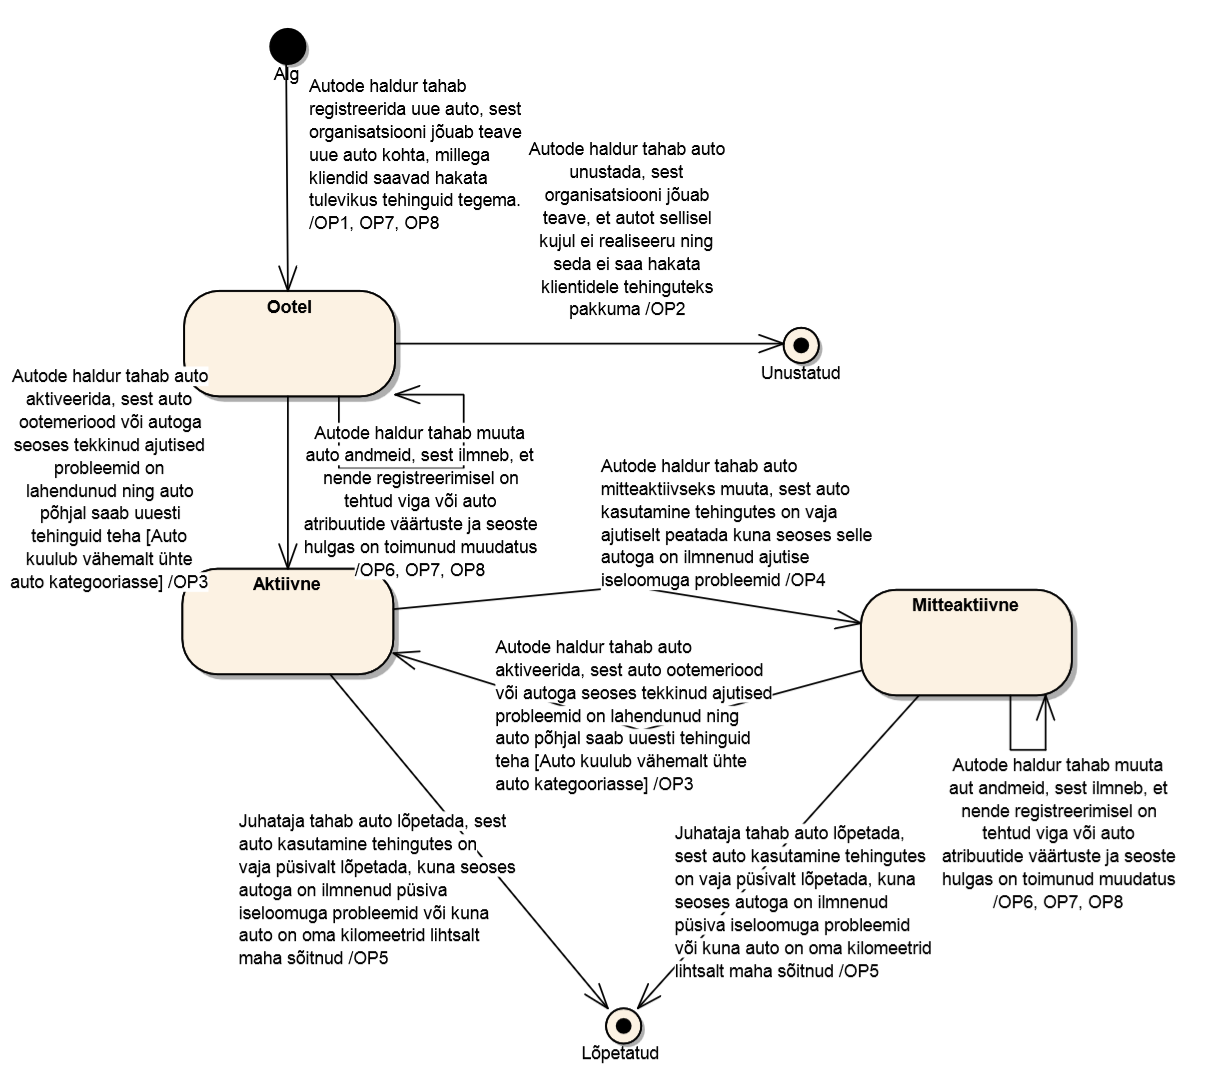
\includegraphics[scale=0.5]{joonis4}
	\caption{\textbf{Joonis 4 Auto seisundidiagramm}}
\end{figure}

\section(CRUD maatriks)
Tabel 7 olev CRUD maatriks esitatakse olemitüüpide ja kasutusjuhtude täpsusega. Maatriksi veergudele vastavad kasutusjuhud ja ridadele olemitüübid. \\ \hfill

\sethlcolor{orange}\hl{Oranzil} taustal on esitatud olemitüübid, mis kuuluvad vaadeldava allsüsteemi teenindatavasse registrisse. 

\begin{figure}[H]
	\caption{\textbf{Tabel 7 CRUD maatriks}}
	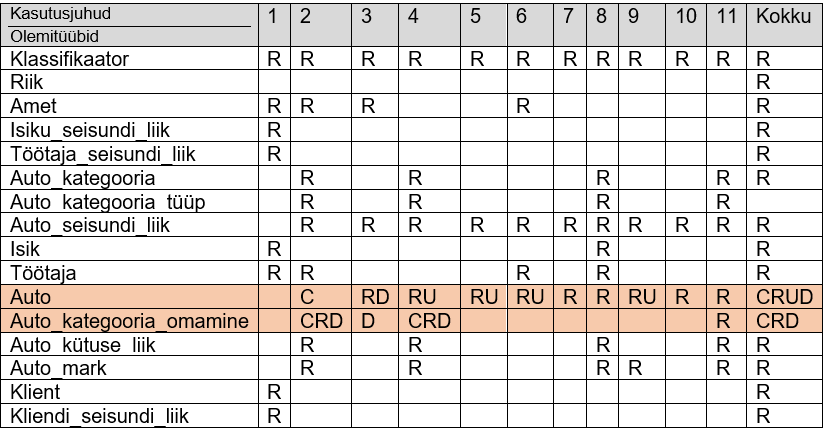
\includegraphics[scale=1]{tabel7}
\end{figure}

\begin{enumerate}
\item Tuvasta kasutaja
\item  Registreeri auto
\item  Unusta auto
\item  Muuda auto andmeid
\item  Aktiveeri auto
\item  Muuda auto mitteaktiivseks
\item  Vaata kõiki ootel või mitteaktiivseid autosid
\item  Vaata kõiki autosid
\item  Lõpeta auto
\item  Vaata auto koondaruannet
\item  Vaata aktiivseid autosid
\end{enumerate}


\chapter{Füüsiline disain}
Selles peatükis esitatakse mudel, mis kirjeldab autode funktsionaalse allsüsteemi toimimiseks vajalike registrite tehnilist lahendust MS Access andmebaasisüsteemis.
\section{Autode funktsionaalse allsüsteemi vajatavate registrite füüsiline disain}

\begin{figure}[H]
	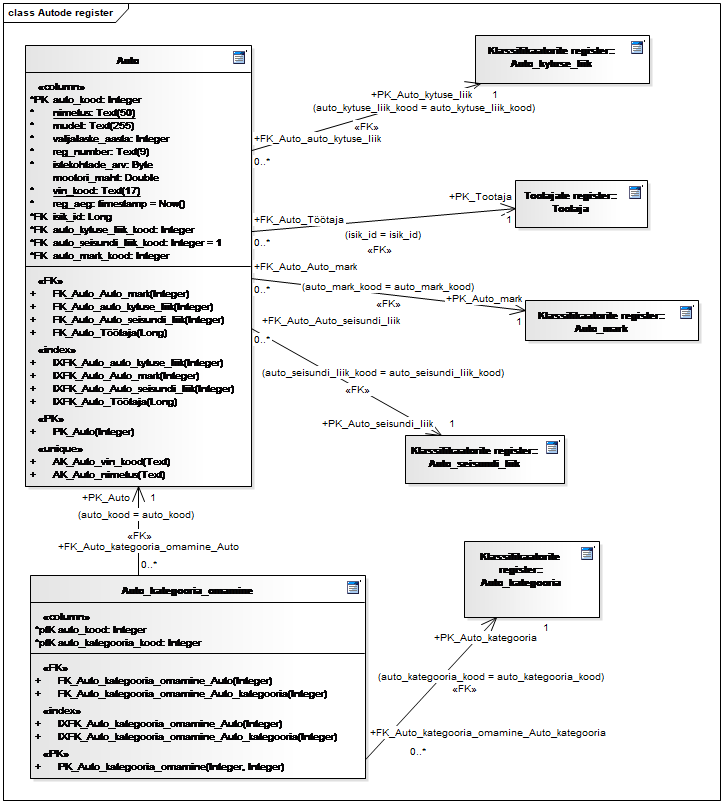
\includegraphics[scale=1]{joonis10}
	\caption{\textbf{Joonis 10. Autode registri füüsilise disaini andmebaasi diagramm}}
\end{figure}

\begin{figure}[H]
	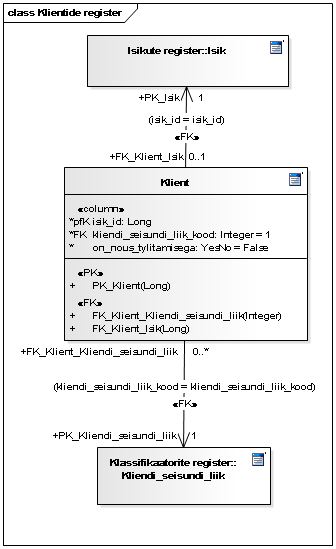
\includegraphics[scale=1]{joonis11}
	\caption{\textbf{Joonis 11. Klientide registri füüsilise disaini andmebaasi diagramm}}
\end{figure}
	
\begin{figure}[H]
	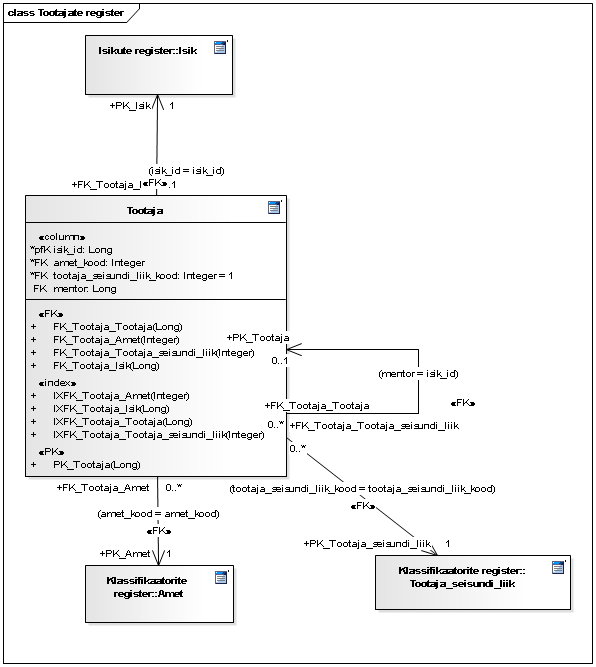
\includegraphics[scale=1]{joonis12}
	\caption{\textbf{Joonis 12. Töötajate registri füüsilise disaini andmebaasi diagramm.}}
\end{figure}

\begin{figure}[H]
	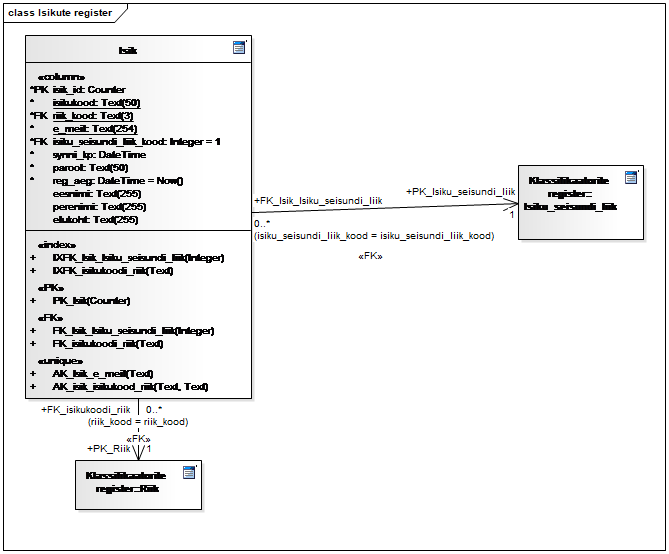
\includegraphics[scale=1]{joonis13}
	\caption{\textbf{Joonis 13. Isikute registri füüsilise disaini andmebaasi diagramm.}}
\end{figure}

\begin{figure}[H]
	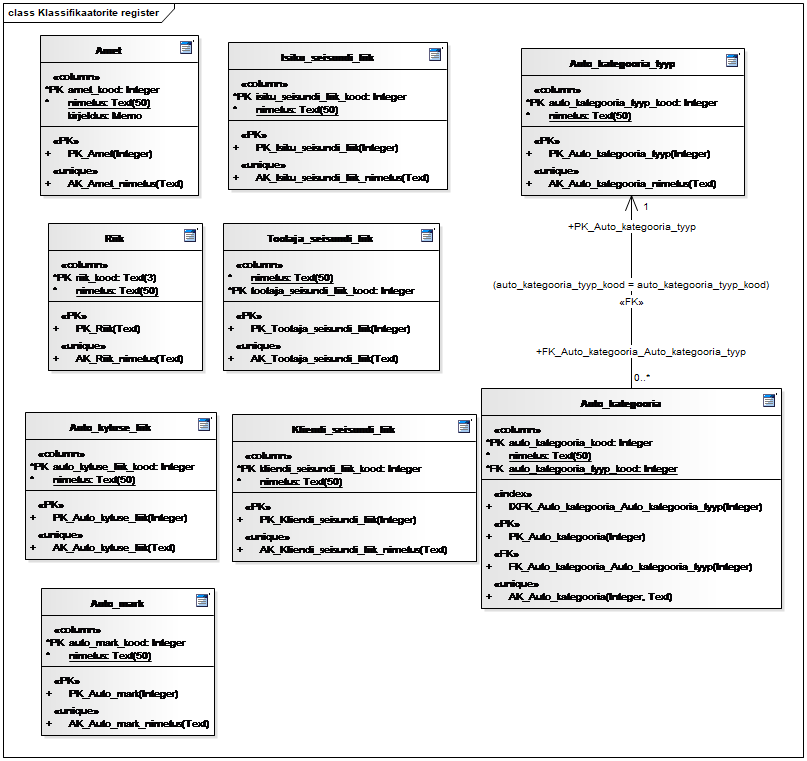
\includegraphics[scale=1]{joonis14}
	\caption{\textbf{Joonis 14. Klassifikaatorite registri füüsilise disaini andmebaasi diagramm.}}
\end{figure}

\chapter{Kasutatud materjalid}
\begin{enumerate}
	\item 1autorent [WWW] http://www.1autorent.ee/esileht (10.03.2017)
	\item AKIT. Andmekaitse ja infoturbe seletussõnastik. [WWW] http://akit.cyber.ee/   (29.01.2017)
	\item Andmebaasid I õppematerjalid. [WWW] http://maurus.ttu.ee (29.01.2017)
	\item Andmebaaside projekti tegemise mall. [WWW] http://maurus.ttu.ee (29.01.2017)
	\item AutoCheck. What is a vehicle identification number (VIN)? [WWW] https://www.autocheck.com/vehiclehistory/autocheck/en/vinbasics (29.08.2018)
	\item Country Codes - ISO 3166 [WWW] http://www.iso.org/iso/home/standards/country\_codes.htm (29.01.2017)
	\item Chisholm, M. (2000). Managing Reference Data in Enterprise Databases: Binding Corporate Data to the Wider World. Morgan Kaufmann.
	\item Eesti Statistika. Riikide ja territooriumide klassifikaator 2013v1. [WWW] http://metaweb.stat.ee/view\_xml\_multi\_code.htm?id=3477719\&siteLanguage=ee (29.01.2017)
	\item ESTERM [WWW] http://termin.eki.ee/esterm/ (29.01.2017)
	\item Hansarent [WWW] http://www.hansarent.ee/en/ (10.03.2017)
	\item Isikuandmete kaitse seadus. [WWW] https://www.riigiteataja.ee/akt/130122010011?leiaKehtiv (29.01.2017)
	12.	Infosüsteemide turvameetmete süsteem. Vabariigi Valitsuse 20.12 2007. a määrus nr 252. Elektrooniline Riigi Teataja.
	[WWW] https://www.riigiteataja.ee/akt/13125331?leiaKehtiv (29.01.2017)
	\item Registreerimismärgid. [WWW] https://www.mnt.ee/et/soiduk/registreerimismargid#tab-1 (06.09.2018)
	\item Schema. Car. [WWW] https://schema.org/Car (13.05.2017)
	\item Vikipeedia. Auto. [WWW] https://et.wikipedia.org/wiki/Auto (25.05.2017)
	\item Vikipeedia. Riik. [WWW] https://et.wikipedia.org/wiki/Riik (29.01.2017) 
	\item Wikipedia. Car model. [WWW] https://en.wikipedia.org/wiki/Car\_model (29.08.2018)
\end{enumerate}
\end{document}